% !TEX root = thesis.tex

\subsection{Hard processes}
\subsubsection{pQCD factorization}


%\begin{figure}[htb]
%\centering
%\includegraphics[width=0.5\textwidth]{pics/QCDLO}
%\caption[QCD Leading Order]{The basic pQCD processes and their quadratic matrix elements}
%\label{fig:qcdlo2}
%\end{figure}





The term Hard Scattering is used in connection with the scattering of two point-like constituents (partons) of colliding nucleons, when the momentum transfer $Q^2$ is large ($Q \gg \Lambda_{\mathrm{QCD}}$). Figure ~\ref{fig:scattering} shows the incoming partons, quarks or gluons, as they exchange a space-like virtual gluon and produce two highly virtual outgoing partons. The outgoing partons will eventually fragment into collimated showers of partons, referred to as jets.

\begin{figure}[htb]
\centering
\documentclass{standalone}
\usepackage{tikz}
\usepackage{xcolor}
\usetikzlibrary{shapes,arrows}
\usetikzlibrary{trees}
\usetikzlibrary{shadows.blur}
\usetikzlibrary{positioning}
\usetikzlibrary{decorations.pathmorphing}
\usetikzlibrary{decorations.markings}
\begin{document}

\tikzset{
photon/.style={decorate, decoration={snake}, draw=red},
particlearrow/.style={draw=blue, postaction={decorate},
    decoration={markings,mark=at position .5 with {\arrow[draw=black]{>}}}},
antiparticlearrow/.style={draw=blue, postaction={decorate},
    decoration={markings,mark=at position .5 with {\arrow[draw=black]{>}}}},
particle/.style={draw=blue},
antiparticle/.style={draw=blue},
gluon/.style={decorate, draw=orange,
    decoration={coil,amplitude=4pt, segment length=5pt}}
 }
 
 
 
\tikzstyle{proton} = [ellipse, draw=black, text centered, fill=orange!20, minimum height=3em, blur shadow = {shadow blur steps=5},minimum width=1em ] 
\begin{tikzpicture}[node distance=1cm and 1.5cm]
\coordinate[] (p1);
\node[proton, right of=p1]  (proton)  {};
\coordinate[below right=-0.05cm and 0.02cm of proton] (aux1);
\coordinate[above right=-0.05cm and 0.02cm of proton] (aux2);
\coordinate[below right=0.0cm and 2cm of aux1] (vertex1);
\coordinate[right=2cm of aux2] (aux4);
\coordinate[right=2cm of proton] (aux5);
\coordinate[right=2cm of aux4] (spec1);
\coordinate[right=2cm of aux5] (spec2);

\coordinate[below right=1.5cm and 0.5cm of vertex1] (vertex2);

\coordinate[below right=0.0cm and 2cm of vertex2] (b1);
\node[proton, below right=-0.05cm and 0.02cm of b1] (proton2) {};
\coordinate[left=2cm of proton2] (aux6);
\coordinate[below left=-0.05cm and 0.02cm of proton2] (b2);
\coordinate[left=2cm of b2] (aux7);
\coordinate[left=2cm of aux7] (spec3);
\coordinate[left=2cm of aux6] (spec4);
\coordinate[right of=proton2] (p2);
\coordinate[above right=1cm and 1cm of vertex1] (jet1);
\coordinate[below left=1cm and 1cm of vertex2] (jet2);


%Jet cones
\coordinate[above right=1cm and 0.5cm of jet1] (cone11);
\coordinate[above right=0.5cm and 1cm of jet1, label={right:Jet}] (cone12);
\draw[particle] (jet1) -- (cone11);
\draw[particle] (jet1) -- (cone12);
\draw[blue] (cone11) to[out=45,in=45]  (cone12);
\draw[blue] (cone11) to[out=225,in=225] (cone12);

\coordinate[below left=1cm and 0.5cm of jet2] (cone21);
\coordinate[below left=0.5cm and 1cm of jet2, label={left:Jet}] (cone22);
\draw[particle] (jet2) -- (cone21);
\draw[particle] (jet2) -- (cone22);
\draw[blue] (cone21) to[out=45,in=45]  (cone22);
\draw[blue] (cone21) to[out=225,in=225] (cone22);

\draw[particlearrow] (p1) -- node[label=above:$P_A$] {} (proton); 
\draw[particlearrow] (aux1) -- node[label=below:$x_a$] {} (vertex1); 
\draw[particlearrow] (aux2) -- (aux4); 
\draw[particlearrow] (proton) -- (aux5);
\draw[particle] (aux4) -- (spec1);
\draw[particle] (aux5) -- (spec2);
\draw[particle] (aux7) -- (spec3);
\draw[particle] (aux6) -- (spec4);
\draw[particle] (vertex1) -- (jet1);
\draw[particle] (vertex2) -- (jet2);

\draw[gluon] (vertex1) -- node[label=right:$q$] {} (vertex2);
\draw[particlearrow] (b1) -- node[label=above:$x_b$] {} (vertex2);
\draw[particlearrow] (b2) -- (aux7);
\draw[particlearrow] (proton2) -- (aux6);

\draw[particlearrow] (p2) -- node[label=above:$P_B$] {} (proton2);




\end{tikzpicture}



\end{document}

%\includegraphics[width=0.5\textwidth]{pics/ink}
\caption[Hard scattering]{Schematic view of hard scattering process between 2 protons, producing 2 jets}
\label{fig:scattering}
\end{figure}

Historically one would study hard scatterings foremost with inclusive hadron spectra. In this context hadron production from hard scatterings can be factorised into three components; the parton distribution functions $f_a$, $f_b$ that give the probability of getting a parton with momentum fraction $x$ of the proton, the cross section of the elementary scattering $ab\rightarrow cd$,  and the fragmentation functions that give the probability of getting hadron $h$ from the parton.

\begin{equation}
\frac{\mathrm{d} \sigma^h_{pp}}{\mathrm{d}y\mathrm{d}^2\pt{}} = K \Sigma_{abcd}\int \mathrm{d}x_a \mathrm{d}x_b f_a\left(x_a,Q^2\right) f_b\left(x_b, Q^2\right) \frac{\mathrm{d} \sigma}{\mathrm{d}t}\left(ab\rightarrow cd \right)\frac{D_{h/c}^0}{\pi z_c},
\end{equation}

\noindent where 

\begin{equation}
x_{a,b} = \frac{\left| p_{a,b} \right|}{\left| p_{proton} \right|}.
\end{equation}


Parton distribution functions will be discussed further in the following section. The elementary cross section $ab\rightarrow cd$ can be calculated from QCD. A summary of the first order $2\rightarrow2$ processes in QCD is shown in Fig. ~\ref{fig:qcdlo}. 

The final component in the factorization, fragmentation functions, describe the distribution of the fractional momenta of fragments radiated from the outgoing parton.  In a leading order picture, it can be interpreted as the probability that the observed final state originates from a given parton~\cite{Metz:2016swz}. Like the PDFs they are non-perturbative and must be determined experimentally. The measurement is usually performed in $e^+ e^-$ collisions where the kinematics are better controlled. 


%
%\begin{figure}
%\centering
%\includegraphics[width=0.9\textwidth]{pics/Showering}
%\caption[Jet showering]{REPLACE FIGURE An illustration of jet showering. The highly virtual parton from the hard scattering will produce a shower of softer partons. When the virtuality is low enough the shower will go through a hadronisation process that produces the hadrons, which will be eventually observed in the detector. }
%\label{fig:highpt}
%\end{figure}



\begin{figure}[htb]
\centering
\documentclass{standalone}
\usepackage{tikz}
\usepackage{array}
\usetikzlibrary{shapes,arrows}
\usetikzlibrary{trees}
\usetikzlibrary{shadows.blur}
\usetikzlibrary{positioning}
\usetikzlibrary{decorations.pathmorphing}
\usetikzlibrary{decorations.markings}
\begin{document}
\newcommand{\centered}[1]{\begin{tabular}{l} #1 \end{tabular}}

\tikzset{
photon/.style={decorate, decoration={snake}, draw=red},
particlearrow/.style={draw=black, postaction={decorate},
    decoration={markings,mark=at position .5 with {\arrow[draw=black]{>}}}},
antiparticlearrow/.style={draw=black, postaction={decorate},
    decoration={markings,mark=at position .5 with {\arrow[draw=black]{>}}}},
particle/.style={draw=black},
antiparticle/.style={draw=blue},
gluon/.style={decorate, draw=black,
    decoration={coil,amplitude=2pt, segment length=3pt}}
 }
 
%\begin{tabular}{ >{\centering\arraybackslash} m{2cm} >{\centering\arraybackslash} m{2cm} >{\centering\arraybackslash} m{8cm}}
\begin{tabular}{ c c c}

\begin{tabular}{c}
$qq' \rightarrow qq' $ \\
$\bar q q' \rightarrow \bar qq' $
\end{tabular} 
& $\frac{4}{9}\frac{\hat s^2+\hat u^2}{\hat t^2}$

&
\centered{

 \begin{tikzpicture}[node distance=1cm and 1.5cm]
\coordinate[] (e1);
\coordinate[right=1cm of e1] (aux1);
\coordinate[right=1cm of aux1] (e2);
\coordinate[below=1cm of aux1] (aux2);
\coordinate[left=1cm of aux2] (e3);
\coordinate[right=1cm of aux2] (e4);

\draw[particle] (e1) -- (aux1);
\draw[particle] (aux1) -- (e2);
\draw[particle] (e3) -- (aux2);
\draw[particle] (aux2) -- (e4);
\draw[gluon] (aux2) -- node[label=left:$t$] {} (aux1);
\end{tikzpicture} 

}
 \\
$qq \rightarrow qq$ & $\frac{4}{9}\left( \frac{\hat s^2+\hat u^2}{\hat t^2} + \frac{\hat s^2+\hat u^2}{\hat t^2}  \right) - \frac{8}{27}\frac{\hat s^2}{\hat u \hat t}$ &
\centered{

\begin{tikzpicture}[node distance=1cm and 1.5cm]
\coordinate[] (e1);
\coordinate[right=1cm of e1] (aux1);
\coordinate[right=1cm of aux1] (e2);
\coordinate[below=1cm of aux1] (aux2);
\coordinate[left=1cm of aux2] (e3);
\coordinate[right=1cm of aux2] (e4);

\draw[particlearrow] (e1) -- (aux1);
\draw[particlearrow] (aux1) -- (e2);
\draw[particlearrow] (e3) -- (aux2);
\draw[particlearrow] (aux2) -- (e4);
\draw[gluon] (aux2) -- node[label=left:$t$] {} (aux1);
\end{tikzpicture} 

\begin{tikzpicture}[node distance=1cm and 1.5cm]
\coordinate[] (e1);
\coordinate[right=1cm of e1] (aux1);
\coordinate[right=1cm of aux1] (e2);
\coordinate[below=1cm of aux1] (aux2);
\coordinate[left=1cm of aux2] (e3);
\coordinate[right=1cm of aux2] (e4);

\draw[particlearrow] (e1) -- (aux1);
\draw[particle] (aux1) -- (e4);
\draw[particlearrow] (e3) -- (aux2);
\draw[particle] (aux2) -- (e2);
\draw[gluon] (aux2) -- node[label=left:$u$] {} (aux1);
\end{tikzpicture}
}
\\
$\bar q q \rightarrow \bar q' q'$ & $\frac{4}{9}\frac{\hat t^2+\hat u^2}{\hat s^2}$ &
\centered{
\begin{tikzpicture}[node distance=1cm and 1.5cm]
\coordinate[] (e1);
\coordinate[below right=0.7cm of e1] (aux1);
\coordinate[right=1cm of aux1] (aux2);
\coordinate[above right=0.7cm of aux2] (e2);
\coordinate[below left=0.7cm of aux1] (e3);
\coordinate[below right=0.7cm of aux2] (e4);

\draw[antiparticlearrow] (aux1) -- (e1);
\draw[antiparticlearrow] (e2) -- (aux2);
\draw[particlearrow] (e3) -- (aux1);
\draw[particlearrow] (aux2) -- (e4);
\draw[gluon] (aux2) -- node[label=above:$s$] {} (aux1);
\end{tikzpicture}
}
\\
$\bar q q \rightarrow \bar q q$ & $\frac{4}{9}\left( \frac{\hat s^2+\hat u^2}{\hat t^2} + \frac{\hat t^2+\hat u^2}{\hat s^2}  \right) - \frac{8}{27}\frac{\hat u^2}{\hat s \hat t}$ &
\centered{

\begin{tikzpicture}[node distance=1cm and 1.5cm]
\coordinate[] (e1);
\coordinate[below right=0.7cm of e1] (aux1);
\coordinate[right=1cm of aux1] (aux2);
\coordinate[above right=0.7cm of aux2] (e2);
\coordinate[below left=0.7cm of aux1] (e3);
\coordinate[below right=0.7cm of aux2] (e4);

\draw[antiparticlearrow] (aux1) -- (e1);
\draw[antiparticlearrow] (e2) -- (aux2);
\draw[particlearrow] (e3) -- (aux1);
\draw[particlearrow] (aux2) -- (e4);
\draw[gluon] (aux2) -- node[label=above:$s$] {} (aux1);
\end{tikzpicture}
\begin{tikzpicture}[node distance=1cm and 1.5cm]
\coordinate[] (e1);
\coordinate[right=1cm of e1] (aux1);
\coordinate[right=1cm of aux1] (e2);
\coordinate[below=1cm of aux1] (aux2);
\coordinate[left=1cm of aux2] (e3);
\coordinate[right=1cm of aux2] (e4);

\draw[antiparticlearrow] (e2) -- (aux1);
\draw[antiparticlearrow] (aux1) -- (e1);
\draw[particlearrow] (e3) -- (aux2);
\draw[particlearrow] (aux2) -- (e4);
\draw[gluon] (aux2) -- node[label=left:$t$] {} (aux1);
\end{tikzpicture} 
}
\\
$\bar q q \rightarrow gg$ & $\frac{32}{27}\frac{\hat u^2+\hat t^2}{\hat u \hat t} - \frac{8}{3}\frac{\hat u^2 + \hat t^2}{\hat s^2}$ &
\centered{

\begin{tikzpicture}
\coordinate[] (e1);
\coordinate[below right=0.7cm of e1] (aux1);
\coordinate[right=1cm of aux1] (aux2);
\coordinate[above right=0.7cm of aux2] (e2);
\coordinate[below left=0.7cm of aux1] (e3);
\coordinate[below right=0.7cm of aux2] (e4);

\draw[antiparticlearrow] (aux1) -- (e1);
\draw[gluon] (aux2) -- (e2);
\draw[particlearrow] (e3) -- (aux1);
\draw[gluon] (aux2) -- (e4);
\draw[gluon] (aux2) -- node[label=above:$s$] {} (aux1);
\end{tikzpicture}
}
\\
$gg \rightarrow \bar q q$ & $\frac{1}{6}\frac{\hat u^2+\hat t^2}{\hat u \hat t} - \frac{3}{8}\frac{\hat u^2 + \hat t^2}{\hat s^2}$ &
\centered{

\begin{tikzpicture}
\coordinate[] (e1);
\coordinate[below right=0.7cm of e1] (aux1);
\coordinate[right=1cm of aux1] (aux2);
\coordinate[above right=0.7cm of aux2] (e2);
\coordinate[below left=0.7cm of aux1] (e3);
\coordinate[below right=0.7cm of aux2] (e4);

\draw[gluon] (e1) -- (aux1);
\draw[antiparticlearrow] (e2) -- (aux2);
\draw[gluon] (e3) -- (aux1);
\draw[particlearrow] (aux2) -- (e4);
\draw[gluon] (aux2) -- node[label=above:$s$] {} (aux1);
\end{tikzpicture}
}
\\

$q g  \rightarrow qg $ & $\frac{4}{9}\frac{\hat u^2+\hat s^2}{\hat u \hat s} + \frac{\hat u^2 + \hat s^2}{\hat t^2}$ &
\centered{

\begin{tikzpicture}
\coordinate[] (e1);
\coordinate[below right=0.7cm of e1] (aux1);
\coordinate[right=1cm of aux1] (aux2);
\coordinate[above right=0.7cm of aux2] (e2);
\coordinate[below left=0.7cm of aux1] (e3);
\coordinate[below right=0.7cm of aux2] (e4);

\draw[gluon] (e1) -- (aux1);
\draw[gluon] (aux2) -- (e2);
\draw[particlearrow] (e3) -- (aux1);
\draw[particlearrow] (aux2) -- (e4);
\draw[particlearrow] (aux1) -- node[label=above:$s$] {} (aux2);
\end{tikzpicture}

\begin{tikzpicture}
\coordinate[] (e1);
\coordinate[below right=0.7cm of e1] (aux1);
\coordinate[right=1cm of aux1] (aux2);
\coordinate[above right=0.7cm of aux2] (e2);
\coordinate[below left=0.7cm of aux1] (e3);
\coordinate[below right=0.7cm of aux2] (e4);

\draw[gluon] (e1) -- (aux2);
\draw[gluon] (aux1) -- (e2);
\draw[particlearrow] (e3) -- (aux1);
\draw[particlearrow] (aux2) -- (e4);
\draw[particlearrow] (aux1) -- node[label=below:$s$] {} (aux2);
\end{tikzpicture}
\begin{tikzpicture}[node distance=1cm and 1.5cm]
\coordinate[] (e1);
\coordinate[right=1cm of e1] (aux1);
\coordinate[right=1cm of aux1] (e2);
\coordinate[below=1cm of aux1] (aux2);
\coordinate[left=1cm of aux2] (e3);
\coordinate[right=1cm of aux2] (e4);

\draw[gluon] (e1) -- (aux1);
\draw[gluon] (aux1) -- (e2);
\draw[particlearrow] (e3) -- (aux2);
\draw[particlearrow] (aux2) -- (e4);
\draw[gluon] (aux2) -- node[label=left:$t$] {} (aux1);
\end{tikzpicture} 
}
\\
$g g  \rightarrow gg $ & $\frac{9}{2}\left(3- \frac{\hat u \hat t}{\hat s^2}  - \frac{\hat u \hat s}{\hat t^2} -\frac{\hat s \hat t}{\hat u^2}\right)$ &
\centered{
\begin{tikzpicture}[node distance=1cm and 1.5cm]
\coordinate[] (e1);
\coordinate[right=1cm of e1] (aux1);
\coordinate[right=1cm of aux1] (e2);
\coordinate[below=1cm of aux1] (aux2);
\coordinate[left=1cm of aux2] (e3);
\coordinate[right=1cm of aux2] (e4);

\draw[gluon] (e1) -- (aux1);
\draw[gluon] (aux1) -- (e2);
\draw[gluon] (e3) -- (aux2);
\draw[gluon] (aux2) -- (e4);
\draw[gluon] (aux2) -- node[label=left:$t$] {} (aux1);
\end{tikzpicture} 
\begin{tikzpicture}
\coordinate[] (e1);
\coordinate[below right=0.7cm of e1] (aux1);
\coordinate[right=1cm of aux1] (aux2);
\coordinate[above right=0.7cm of aux2] (e2);
\coordinate[below left=0.7cm of aux1] (e3);
\coordinate[below right=0.7cm of aux2] (e4);

\draw[gluon] (e1) -- (aux1);
\draw[gluon] (aux2) -- (e2);
\draw[gluon] (e3) -- (aux1);
\draw[gluon] (aux2) -- (e4);
\draw[gluon] (aux2) -- node[label=above:$s$] {} (aux1);
\end{tikzpicture}

\begin{tikzpicture}[node distance=1cm and 1.5cm]
\coordinate[] (e1);
\coordinate[right=1cm of e1] (aux1);
\coordinate[right=1cm of aux1] (e2);
\coordinate[below=1cm of aux1] (aux2);
\coordinate[left=1cm of aux2] (e3);
\coordinate[right=1cm of aux2] (e4);

\draw[gluon] (e1) -- (aux1);
\draw[gluon] (aux1) -- (e4);
\draw[gluon] (e3) -- (aux2);
\draw[gluon] (aux2) -- (e2);
\draw[gluon] (aux2) -- node[label=left:$u$] {} (aux1);
\end{tikzpicture}

\begin{tikzpicture}
\coordinate[] (e1);
\coordinate[below right=0.7cm of e1] (aux1);
\coordinate[above right=0.7cm of aux1] (e2);
\coordinate[below left=0.7cm of aux1] (e3);
\coordinate[below right=0.7cm of aux1] (e4);

\draw[gluon] (e1) -- (aux1);
\draw[gluon] (aux1) -- (e2);
\draw[gluon] (e3) -- (aux1);
\draw[gluon] (aux1) -- (e4);
\end{tikzpicture}
}


\end{tabular}
\end{document}
\caption[QCD Leading Order]{The basic pQCD processes and their quadratic matrix elements}
\label{fig:qcdlo}
\end{figure}



\subsubsection*{Parton Distribution Function}
Parton Distribution Functions (PDFs) $f_a\left(x\right)$ give the differential probability for parton $a$ to carry momentum fraction $x$ of the proton momentum. %PDFs  are extracted from comprehensive global analysis of experimental results from a variety of fixed-target and collider experiments.
As the PDFs cannot be calculated from first principles they are measured in Deeply Inelastic Scattering (DIS) experiments~\cite{missing} and are extrapolated to the relevant momentum scales using the Dokshitzer-Gribov-Lipatov-Altarelli-Parisi (DGLAP) evolution scheme ~\cite{Gribov:1972ri,Altarelli:1977zs,Dokshitzer:1977sg}  %~\ref{eq:dglap}.

\begin{equation}
\mu_\mathrm{F}^2 \frac{\partial f_i\left(x,\mu_{\mathrm{F}}^2 \right)}{\partial \mu_{\mathrm{F}}^2} = \Sigma_j \frac{\alpha_s\left(\mu_{\mathrm{F}}\right)}{2{pi}} \int _x^1 \frac{\mathrm{d}z}{z} P_{ij}(z) f_j\left(\frac{x}{z},\mu_{\mathrm{F}}^2\right),
\label{eq:dglap}
\end{equation}



\noindent where $\mu_{\mathrm{F}}$ is a factorization scale. The splitting functions $P_{ij}$ describe a probability to radiate parton $i$ from parton $j$ as a function of the momentum fraction $z$ carried away by the offspring parton. Different theory interpretation and experimental data gives rise to different PDF's. Thus there are several commonly used PDF sets: CTEQ~\cite{cteq}, HERAPDF~\cite{CooperSarkar:2011aa}, PDF4LHC~\cite{Butterworth:2015oua}, etc. %Depending on the data used 

\subsubsection{Jet showering}
\label{sec:shower}
\begin{figure}
\centering
\documentclass{standalone}
\usepackage{tikz}
\usepackage{xcolor}
\usetikzlibrary{shapes,arrows}
\usetikzlibrary{trees}
\usetikzlibrary{shadows.blur}
\usetikzlibrary{positioning}
\usetikzlibrary{decorations.pathmorphing}
\usetikzlibrary{decorations.markings}
\begin{document}
\tikzset{
photon/.style={decorate, decoration={snake}, draw=red},
particlearrow/.style={draw=blue, line width=0.75pt, postaction={decorate},
    decoration={markings,mark=at position .5 with {\arrow[draw=black]{>}}}},
antiparticlearrow/.style={draw=blue, postaction={decorate},
    decoration={markings,mark=at position .5 with {\arrow[draw=black]{>}}}},
particle/.style={draw=blue, line width=0.75pt},
hadron/.style={draw=blue,line width=2pt,postaction={decorate},
    decoration={markings,mark=at position .9 with {\arrow[draw=blue]{>}}}},
antiparticle/.style={draw=blue},
gluon/.style={decorate, draw=orange, line width=0.75pt,
    decoration={coil,amplitude=4pt, segment length=5pt}}
 }
\begin{tikzpicture}
%\draw[step = 4cm, gray, thin] (-3cm,-3cm) grid(8,4cm);

\node[ellipse,draw=orange,fill=orange!20, minimum height=1cm, blur shadow = {shadow blur steps=5},minimum width=2cm] (hard) {};
\coordinate[above=1cm of hard, label=Hard Scattering] (label);
\coordinate[left=1cm of hard] (p1);
\coordinate[above left=1cm and 1cm of hard] (p2);
\coordinate[right=1cm of hard] (p3);
\coordinate[below right=1cm and 1cm of hard] (p4);

\coordinate[above right=1cm and 1.25cm of p3] (vertex1_1);
\coordinate[below right=1cm and 1.25cm of p3]  (vertex1_2);

\coordinate[above right=0.75cm and 1cm of vertex1_1] (vertex2_1);
\coordinate[below right=0.3cm and 1cm of vertex1_1] (vertex2_2);
\coordinate[above right=0.3cm and 1cm of vertex1_2] (vertex2_3);
\coordinate[below right=0.75cm and 1cm of vertex1_2] (vertex2_4);


\coordinate[above right=0.75cm and 1cm of vertex2_1] (vertex3_1);
\coordinate[below right=0.3cm and 1cm of vertex2_1] (vertex3_2);
\coordinate[above right=0.3cm and 1cm of vertex2_2] (vertex3_3);
\coordinate[below right=0.3cm and 1cm of vertex2_2] (vertex3_4);
\coordinate[above right=0.3cm and 1cm of vertex2_3] (vertex3_5);
\coordinate[below right=0.3cm and 1cm of vertex2_3] (vertex3_6);
\coordinate[above right=0.3cm and 1cm of vertex2_4] (vertex3_7);
\coordinate[below right=0.75cm and 1cm of vertex2_4] (vertex3_8);


\draw[particlearrow] (p1) -- (hard);
\draw[particlearrow] (p2) -- (hard);
\draw[particlearrow] (hard) -- (p3);
\draw[particlearrow] (hard) -- (p4);

\draw[particle] (p3) -- (vertex1_2);
\draw[gluon] (p3) -- (vertex1_1);

\draw[particle] (vertex1_1) -- (vertex2_1);
\draw[gluon] (vertex1_1) -- (vertex2_2);
\draw[gluon] (vertex1_2) -- (vertex2_3);
\draw[gluon] (vertex1_2) -- (vertex2_4);

\draw[gluon] (vertex2_1) -- (vertex3_1);
\draw[particle] (vertex2_1) -- (vertex3_2);
\draw[particle] (vertex2_2) -- (vertex3_3);
\draw[particle] (vertex2_2) -- (vertex3_4);
\draw[gluon] (vertex2_3) -- (vertex3_5);
\draw[gluon] (vertex2_3) -- (vertex3_6);
\draw[particle] (vertex2_4) -- (vertex3_7);
\draw[particle] (vertex2_4) -- (vertex3_8);

\node[rectangle,draw=orange, fill=orange!20, below right=-0.5cm and 0cm of vertex3_1,minimum width=1cm, minimum height=6cm,label={below:Hadronisation},blur shadow = {shadow blur steps=5}] (hadr) {};

\coordinate[right=0cm of hadr] (hadron1);
\coordinate[right=2cm of hadron1] (detector1);

\coordinate[above=1.5cm of hadron1] (hadron2);
\coordinate[above=2.5cm of hadron1] (hadron3);
\coordinate[below=1cm of hadron1] (hadron4);
\coordinate[below=2.5cm of hadron1] (hadron5);
\coordinate[right=2cm of hadron2] (detector2);
\coordinate[right=2cm of hadron3] (detector3);
\coordinate[right=2cm of hadron4] (detector4);
\coordinate[right=2cm of hadron5] (detector5);


\draw[hadron] (hadron1) -- node[label=above:Hadrons] {}(detector1);
\draw[hadron] (hadron2) -- (detector2);
\draw[hadron] (hadron3) -- (detector3);
\draw[hadron] (hadron4) -- (detector4);
\draw[hadron] (hadron5) --  (detector5);


\end{tikzpicture}
\end{document}

\caption[Jet showering]{An illustration of jet showering. The highly virtual parton from the hard scattering will produce a shower of softer partons. When the virtuality is low enough the shower will go through a hadronisation process that produces the hadrons, which will be eventually observed in the detector. }
\label{fig:showering}
\end{figure}

More detailed studies of the hard processes require a formulation of the showering process. The full picture is a complicated $2\rightarrow n$ scattering, but it is typically seen as a series of $1\rightarrow2$ splittings with decreasing virtuality following the initial $2\rightarrow 2$ scattering~\cite{newPythiaShower}.

To first order the cascade is governed by the DGLAP evolution equation~\cite{Gribov:1972ri,Altarelli:1977zs,Dokshitzer:1977sg}

\begin{equation}
\mathrm{d} P_a\left(z,Q^2\right) = \frac{\mathrm{d}Q^2}{Q^2}\frac{\alpha_s}{2\pi} P_{a\rightarrow bc}\left(z\right)dz,
\label{eq:dglap}
\end{equation} 

\noindent which gives the differential probability that parton $a$ (mother) will branch to two partons $b$ and $c$ (daughters), at a virtuality scale $Q^2$. Daughter $b$ takes a fraction $z$ of the parton $a$ energy and daughter $c$ takes energy fraction $1-z$. The splittings kernels $P_{a\rightarrow bc}\left(z\right)$ are 
\nopagebreak
\begin{align}
P_\mathrm{q\rightarrow qg}\left(z\right) &= \frac{4}{3}\frac{1+z^2}{1-z} \\
P_\mathrm{g\rightarrow gg}\left(z\right) &= 3\frac{\left(1-z\left(1-z \right) \right)^2}{z\left(1-z\right)} \\
P_\mathrm{g\rightarrow q \bar q}\left(z\right)& = \frac{n_f}{2}\left( z^2+\left(1-z\right)^2\right),
\end{align}

\noindent where $n_f$ is the kinematically allowed number of quark flavours. There is some freedom in how the evolution variable $Q^2$ is chosen. If $Q^2=f\left(z \right) m^2$ and $f\left(z \right)$ is a positive and a smooth function it holds that

\begin{equation}
\frac{\mathrm{d}Q^2}{Q^2}\mathrm{d}z = \frac{\mathrm{d} m^2}{m^2} \mathrm{d}z. 
\end{equation}

Of the Monte Carlo generators used in this thesis \pythia~uses $m^2$ as the evolution variable~\cite{missing}, while HERWIG uses an energy-weighted emission angle $E^2\left(1-\cos\theta\right) \approx \nicefrac{m^2}{z\left(1-z\right)}$~\cite{missing}.

Formally eq~\ref{eq:dglap} corresponds to the emission of an infinite number of partons. However very soft and collinear gluons need not considered and one can introduce an effective cut-off scale $Q_0$, usually taken to be of the order of \unit[1]{\gev}.

Going further one approach is to introduce time ordering, i.e. to decide which of the emissions occurs first. This is done in the form of a Sudakov form factor~\cite{missing}

\begin{equation}
P_a^{no}\left(Q^2_\mathrm{max},Q^2\right) = \exp \left(- \int_{Q^2}^{Q^2_\mathrm{max}}\int_{z_\mathrm{min}}^{z_\mathrm{max}} \mathrm{d} P_a \left(z',Q'^2\right)\right),
\end{equation} 

\noindent which gives the probability that no emissions occur between the initial maximum scale $Q^2_\mathrm{max}$ and a given $Q^2$ and within limits $z_\mathrm{min} < z < z_\mathrm{max}$. Thus the probability for the first branching to occur at $Q^2=Q^2_a$ is given by 
\begin{equation}
\dd \Delta_a\left(z,Q_a^2,Q_\mathrm{max}^2\right)=\mathrm{d}P_a \left(z,Q^2_a\right) P_a^{no}\left(Q^2_\mathrm{max},Q_a^2\right).
\end{equation}

Partons $b$ and $c$ that were produced will further branch with maximum virtuality scale $Q^2_\mathrm{max}$ given by $Q^2_a$. Similarly their daughters will continue branching until the cutoff scale is reached, thus producing a shower. 

\begin{figure}[h]
\centering
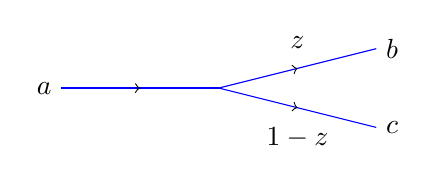
\begin{tikzpicture}
\tikzset{
photon/.style={decorate, decoration={snake}, draw=red},
particlearrow/.style={draw=blue, postaction={decorate},
    decoration={markings,mark=at position .5 with {\arrow[draw=black]{>}}}},
antiparticlearrow/.style={draw=blue, postaction={decorate},
    decoration={markings,mark=at position .5 with {\arrow[draw=black]{>}}}},
particle/.style={draw=blue},
antiparticle/.style={draw=blue},
gluon/.style={decorate, draw=orange,
    decoration={coil,amplitude=4pt, segment length=5pt}}
 }
 
\coordinate[label=left:$a$] (a);
\coordinate[right=2cm of a] (vertex);
\coordinate[above right=0.5cm and 2 cm of vertex,label=right:$b$] (b);
\coordinate[below right=0.5cm and 2 cm of vertex,label=right:$c$] (c);
\draw[particlearrow] (a) -- (vertex);
\draw[particlearrow] (vertex) -- node[label=above:$z$] {} (b);
\draw[particlearrow] (vertex) -- node[label=below:$1-z$] {} (c);
\end{tikzpicture}
\end{figure}




\subsubsection{Soft gluon radiation and angular ordering}

\begin{figure}[tb]
\centering
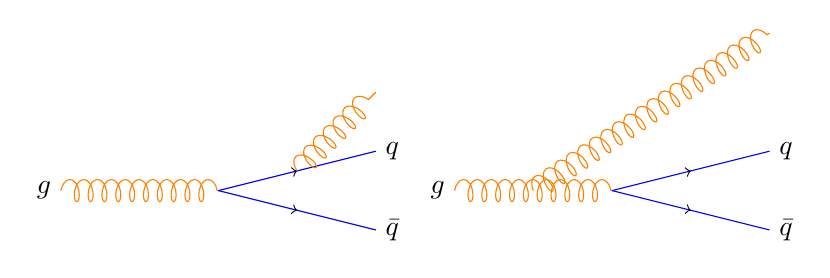
\begin{tikzpicture}[scale = 2]
\tikzset{
photon/.style={decorate, decoration={snake}, draw=red},
particlearrow/.style={draw=blue, postaction={decorate},
    decoration={markings,mark=at position .5 with {\arrow[draw=black]{>}}}},
antiparticlearrow/.style={draw=blue, postaction={decorate},
    decoration={markings,mark=at position .5 with {\arrow[draw=black]{>}}}},
particle/.style={draw=blue},
antiparticle/.style={draw=blue},
gluon/.style={decorate, draw=orange,
    decoration={coil,amplitude=4pt, segment length=5pt}}
 }
\coordinate[label=left:$g$] (a);
\coordinate[right=2cm of a] (vertex);
\coordinate[above right = 0.25cm and 1cm of vertex] (vertex2);
\coordinate[above right=1cm and 1cm of vertex2] (gluon);
\coordinate[above right=0.5cm and 2 cm of vertex,label=right:$q$] (b);
\coordinate[below right=0.5cm and 2 cm of vertex,label=right:$\bar q$] (c);
\draw[gluon] (a) -- (vertex);
\draw[particlearrow] (vertex) --  (b);
\draw[particlearrow] (vertex) --  (c);
\draw[gluon] (vertex2) -- (gluon);

\coordinate[label=left:$g$,right=3cm of vertex] (g2);
\coordinate[right=2cm of g2] (vertex3);
\coordinate[left = 1cm of vertex3] (vertex4);
\coordinate[above right=2cm and 3cm of vertex4] (gluon2);
\coordinate[above right=0.5cm and 2 cm of vertex3,label=right:$q$] (b2);
\coordinate[below right=0.5cm and 2 cm of vertex3,label=right:$\bar q$] (c2);
\draw[gluon] (g2) -- (vertex3);
\draw[particlearrow] (vertex3) --  (b2);
\draw[particlearrow] (vertex3) --  (c2);
\draw[gluon] (vertex4) -- (gluon2);
\end{tikzpicture}

\caption{Soft gluon production}
\label{fig:soft}
\end{figure}

Let us now consider a case where a gluon splits into two quarks, and one of the created quarks emits a soft gluon as seen in Fig.~\ref{fig:soft}. In the laboratory frame the time it takes for a gluon to be emitted from a quark can be estimated to be~\cite{basicsofpqcd}



\begin{equation}
t_\mathrm{emit} \approx \frac{1}{E_q},
\end{equation}


\noindent where the energy of the quark is given by $E_q$. In the rest frame of the quark its energy is given by its virtuality $M_\mathrm{virt}$ and assuming the quark is massless the Lorentz factor between the rest frame the laboratory frame is 

\begin{equation}
\gamma = \frac{E_q}{M_\mathrm{virt}}.
\end{equation}

\noindent Thus the emission time can be written as

\begin{equation}
t_\mathrm{emit} \approx \frac{E_q}{M_\mathrm{virt}^2}  = \frac{E_q}{\left(k+p\right)^2},
\end{equation}
\noindent where $k$ and $p$ are the four-momenta of the gluon and the quark after the gluon emission. This can be written open in the laboratory frame. Through assuming that the end products are massless and Taylor-expanding the resulting cosine term gives a form that expresses the emission time using the opening angle $\theta_\mathrm{kq}$ between the quark and the gluon


\begin{equation}
t_\mathrm{emit} \approx \frac{1}{k\theta_\mathrm{kq}^2}.
\end{equation}


\noindent The transverse wavelength of the emitted gluon is $\lambda_\perp^{-1}=k_\perp\approx k\theta_\mathrm{kq}$. Thus we get

\begin{equation}
t_\mathrm{emit} \approx \frac{\lambda_\perp}{\theta_\mathrm{kq}}.
\end{equation}

\noindent The secondary gluon can only probe the quark of the earlier splitting if the transverse wavelength is smaller than the transverse separation of the produced $\mathrm{q \bar q}$ pair. The transverse separation is given by

\begin{equation}
r_\perp^{\mathrm{q \bar q}} \approx \theta_\mathrm{q \bar q} t_\mathrm{emit} \approx \lambda_\perp \frac{\theta_\mathrm{q \bar q} }{\theta_\mathrm{k q} }.
\end{equation}

\noindent Thus in order for the emission to probe the individual quark, the opening angle of the $\mathrm{q \bar q}$ splitting, $\theta_\mathrm{q \bar q}$, must be larger than $\theta_\mathrm{k q}$. If the opening angle $\theta_\mathrm{k q}$ is larger, the gluon can't distinguish between the quark and the antiquark, so it probes the state of the system before the splitting, i.e. it can be treated like it was emitted from the primary gluon.  

This leads to the angular ordering of soft gluon radiation. Each successive angle must be smaller than the previous one. The effect can be calculated in all orders ~\cite{missing} and in the DGLAP formalism one can select the evolution variable $Q^2$ in a way that ensures angular ordering~\cite{missing} as is done in the Herwig MC generator. In \pythia~8 this is strictly not included, but the transverse momentum ordered showers are as accurate in describing the soft gluon emissions as the angular ordered showers~\cite{eventGenerators}.

%(The soft gluon behaves as if testing the colour charge of the jet as a whole)= As a results to describe the jet evolution in terms of independent sequential parton splittings one has to include the Angular ordering (AO) condition. This is implemented differently in Monte Carlo generators. In \pythia 8 this is strictly not included, but the transverse momentum ordered showers are as accurate in describing the soft gluon emissions as the angular ordered showers~\cite{eventGenerators}. In Herwig angular ordering is a consequence of the choice of the evolution variable.



\subsubsection{Jet hadronisation}
When the virtuality of the shower is low enough, the shower starts to hadronise. In this regime the parton shower reaches a scale close to $\Lambda_{\mathrm{QCD}}$ and the perturbative description is no longer valid. Thus the hadronisation stage must be described in a non-perturbative manner. In general hadronisation is assumed to be universal, i.e. it shouldn't depend on the collision energy or system. 
The most simple scenario that is used in several theory calculations is the so-called local parton-hadron duality~\cite{Azimov1985}. In the local parton-hadron duality hypothesis it is assumed that there exists a low virtuality scale $Q_0$ in which the hadronisation happens, that is independent of the scale of the primary hard process. At this scale the partons are transformed into hadrons, assuming that the flow of momentum and quantum numbers for the hadrons can be directly obtained from those of partons introducing only small normalising constants. 

The next sections will present more complicated hadronisation models used in Monte Carlo generators, \pythia~and Herwig.

\subsubsection*{Lund string model}

One common implementation in MC generators is the Lund string fragmentation algorithm~\cite{ANDERSSON198331}. The string model is based on the fact that in QCD linear confinement is expected over large distances~\cite{eventGenerators}. This can be modelled by imagining a colour flux tube being stretched between the outgoing partons. The left side of Fig. ~\ref{fig:fluxtube} illustrates this point for a $\mathrm{q \bar q}$-pair. The tube is assumed to have a uniform fixed transverse size of about \unit[1]{fm} along its length, which leads to a linearly rising potential $V\left(r\right) = \kappa r$, where the string constant $\kappa$ describes the amount of energy per unit length. A value of $\kappa \approx \unit[1]{\GeVfm} \approx\unit[0.2]{GeV^2}$ can be obtained from hadron mass spectroscopy~\cite{missing}.

The evolution of string fragmentation is illustrated schematically on the right side of Fig.~\ref{fig:fluxtube}. This figure is drawn in a light cone presentation, so the initial quark and antiquark are going to separate directions at the speed of light. The string between them, illustrated in the figure by the red line, stretches until its potential energy becomes high enough that it can break, forming a new quark-antiquark pair. If the original pair was $\mathrm{q \bar q}$ and the new pair $\mathrm{q'\bar q'}$, now two new pairs $\mathrm{q \bar q'}$ and $\mathrm{q'\bar q}$ have formed. As these particles are also moving away from each other, the strings between them can stretch and break, creating yet more pairs. The process continues until the invariant mass of the system connected by the string becomes small enough and a final state meson is formed. 

\begin{figure}
\centering
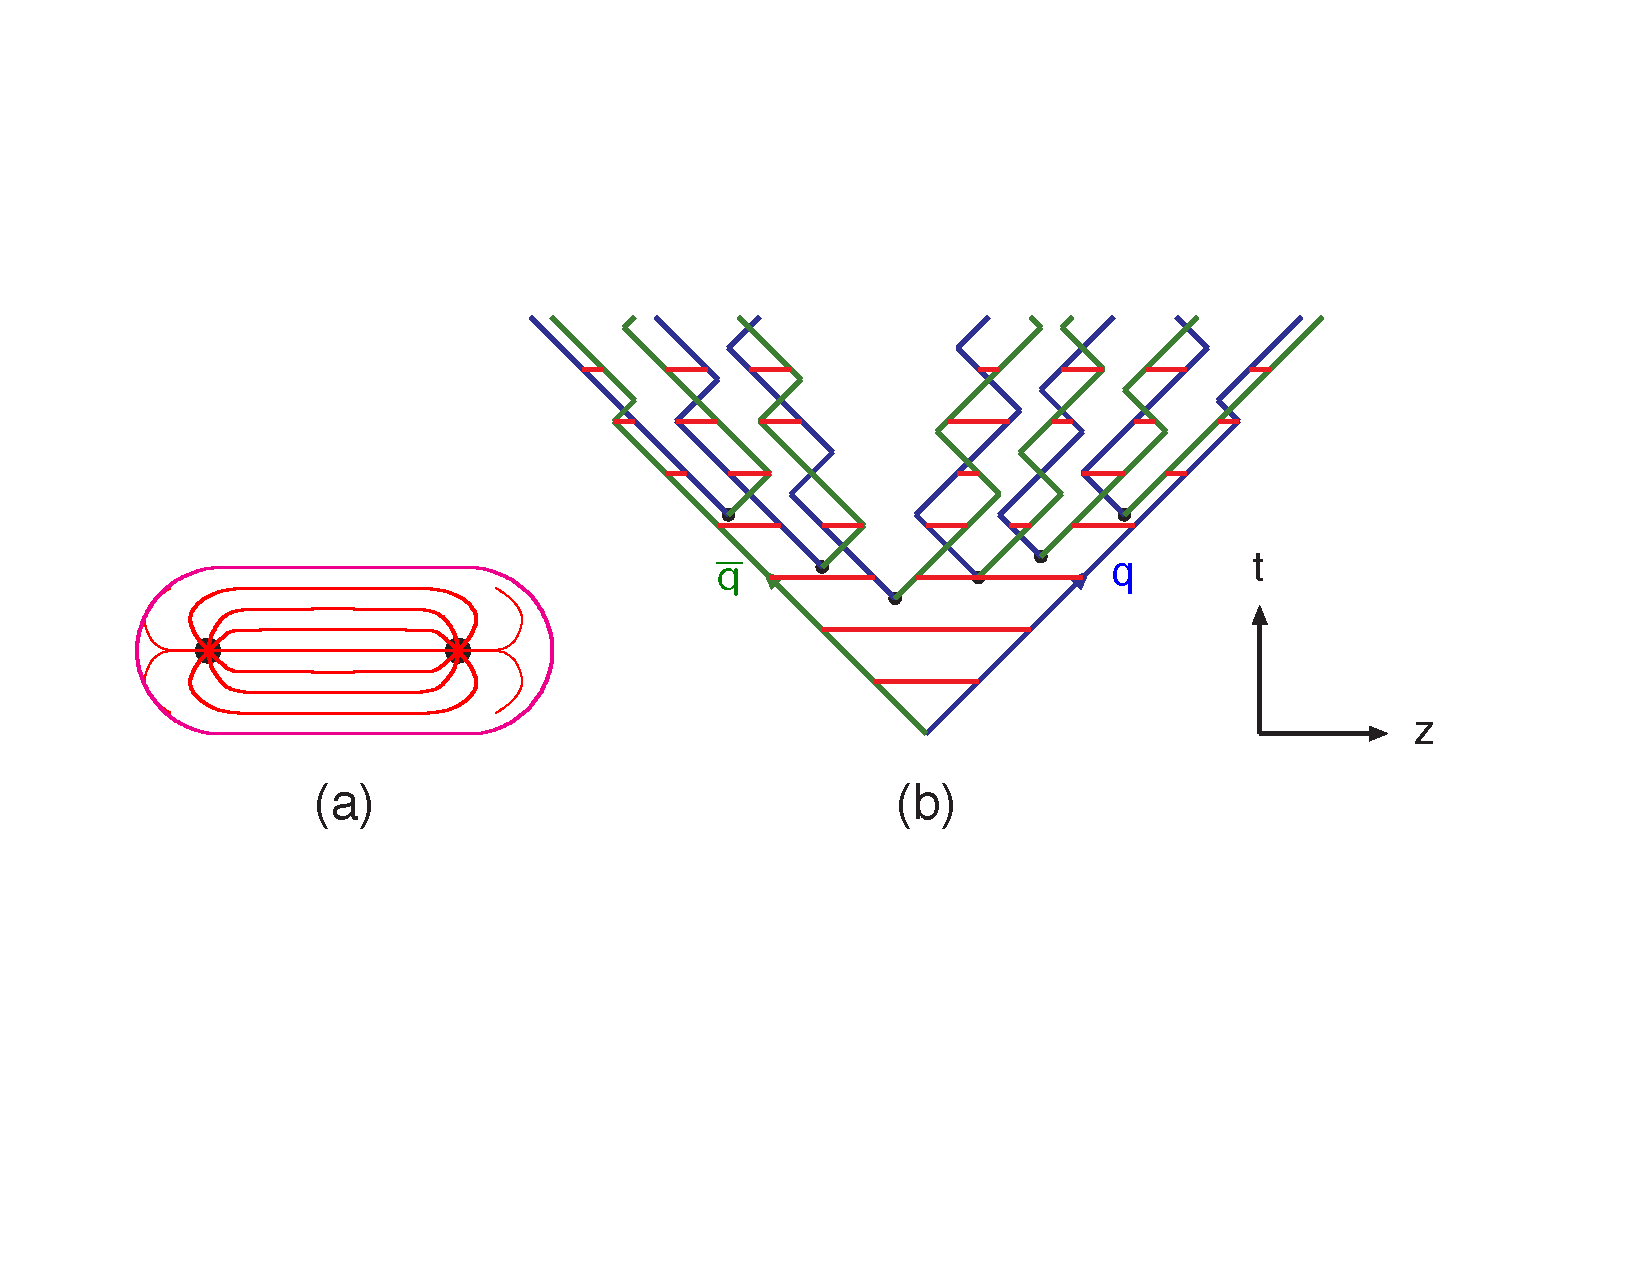
\includegraphics[width=0.75\textwidth]{pics/stringone.pdf}
\caption[]{ (a) A flux tube spanned between a quark and an antiquark. (b) The motion
and breakup of a string system, with the two transverse degrees of freedom suppressed
(diagonal lines are (anti)quarks, horizontal ones snapshots of the string field) \cite{eventGenerators}.
 }
\label{fig:fluxtube}
\end{figure}

To mathematically model the string one can use a massless relativistic string with no transverse degrees of freedom. The gluons are represented as energy and momentum carrying kinks on the string with incoherent sums of one colour charge and one anticolour charge. When this string breaks, it is classically required that the created quark and antiquark are produced at a certain distance if they are to have any mass or transverse momentum. However, taking into account quantum mechanics, the pair must be created at one point and then tunnel out to the classically allowed region. Thus the probability to create a new quark-antiquark pair becomes proportional to the tunnelling probability~\cite{ANDERSSON198331}.


\begin{equation}
P_\mathrm{tunnelling} \propto \exp \left(\frac{-\pi m_\perp^2}{\kappa} \right) = \exp \left(\frac{-\pi m^2}{\kappa} \right) \left(\frac{-\pi p_\perp^2}{\kappa} \right),
\end{equation}

\noindent where the transverse mass $m_\perp$ is defined as $m_\perp^2 = m^2 + p_\perp ^2$. The transverse momentum is now defined to be transverse to the string axis. This formula gives flavour-independent Gaussian $p_\perp$-distribution for the created $\mathrm{q \bar q}$ pairs.

As explained above the string fragmentation would only produce mesons in the final state, but we know that also baryons are created in the process. In the string fragmentation model baryon production is included by adding a probability that a diquark-antidiquark pair is created instead of a quark-antiquark pair when a string breaks.

The kinematics of each string breaking are determined iteratively. Since there is no natural ordering, the string breaking can be considered in any order and the answer obtained must be the same. One can start from the q leg and work one's way to the $\bar{\mathrm{q}}$ leg, or vice versa. This give a left-right symmetry of the string fragmentation. In the Lund model this is taken into account by defining a symmetric fragmentation function

\begin{equation}
f\left(z\right) \propto \frac{1}{z} \left(1-z\right)^a \exp \left(-\frac{b m_\perp ^2}{z} \right)
\label{eq:symmetric}
\end{equation}

\noindent to break the string into a hadron and a remainder system. Here $z$ is the fraction of light-cone momentum $p^+$ given to the hadron in the string breaking, $m_\perp$ is the transverse mass of the hadron and $a$ and $b$ are tuneable parameters of the model. For heavy quarks this is modified as 

\begin{equation}
f\left(z\right) \propto \frac{1}{z^{1+bm_Q^2}} \left(1-z\right)^a \exp \left(-\frac{b m_\perp ^2}{z} \right).
\label{eq:symmetric2}
\end{equation}

\noindent The process can be thought as follows: first start from the q-leg of a $\mathrm{q \bar{q}}$ system and choose to consider the breaking to new $\mathrm{q' \bar q'}$ pair closest to this leg. Now the breaking will produce a hadron $\mathrm{q \bar{q}'}$ and a remainder system spanning from $\mathrm{q' \bar{q}}$. Then the process is continued until the $\bar{\mathrm{q}}$-leg is reached. A small detail here is that in equation (\ref{eq:symmetric}) it is assumed that the mass of the remainder system is large. Thus some patching up is needed for the last two hadrons coming from a string. The patching up is done such that the place where it happens looks as closely like any other string break as possible.


One additional possibility one must consider is that a string can have such a low mass that it cannot break at all. In this case a single hadron is generated out of the string and if necessary  energy and momentum are exchanged with other partons in the event.

After all the hadrons are produced, the short-lived ones can still decay before the set of final state particles in the simulation is obtained~\cite{missing}


\subsubsection*{Cluster model}
Instead of a string model HERWIG~\cite{herwigManual} uses a cluster model for hadronisation. The advantage of cluster models is that they require a smaller number of parameters than string models. The model is based on the preconfinement property of parton showers, i.e. the colour structure of the shower at any evolution scale $Q_0$ is such that colour singlet combinations of partons can be formed with an asymptotically universal invariant mass distribution. The invariant mass does not depend on the initial hard process scale $Q$, but only on $Q_0$ and the QCD scale $\Lambda _ \mathrm{QCD}$, when $Q \gg Q_0$~\cite{missing}.

The cluster model starts from transforming all gluons non-perturbatively into $\mathrm{q \bar q}$ pairs, which requires that the gluons get a mass, which must be at least twice the lightest quark mass. After the gluons are transformed into quarks, the adjacent colour lines can be clustered together to colour singlet states with mesonic quantum numbers. The momentum of these clusters is defined to be the sum of the momenta of the clustering partons. The principle of colour-preconfinement states that the mass distribution of these clusters is independent of the hard scattering process and its centre-of-mass energy~\cite{herwigManual}. %As the mass distribution is peaked at low masses, the clusters can be regarded as highly excited hadron resonances and decayed into the final state hadrons.

Some of these initial clusters are too heavy to reasonably describe an excited state of a hadron. These must be
split before they are allowed to decay. The cluster $C$ is split if its mass fulfils the condition~\cite{herwigManual}

\begin{equation}
M_C^p \geq M_\mathrm{max}^p  + \left( m_1 + m_2\right)^p,
\label{eq:clustermass}
\end{equation}

\noindent where $m_{1,2}$ are the masses of the constituents partons of the cluster. $M_\mathrm{max}$ and $p$ are parameters given defined the model. These have to be chosen separately for clusters containing light, charmed and bottom quarks. When a cluster splits, a pair of light quarks is generated from the vacuum, which form two new clusters, both containing one quark from the original cluster and one from the newly generated pair. The splitting continues until no clusters with masses fulfilling the equation ~\ref{eq:clustermass} remains.

\begin{figure}
\centering
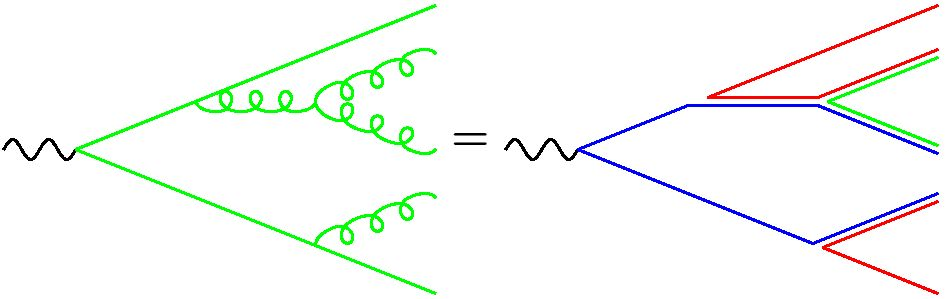
\includegraphics[width=0.75\textwidth]{pics/planar.jpg}
\caption[]{ Colour structure of a parton shower to leading order in Nc.
\cite{eventGenerators} }
\label{fig:colourstructure}
\end{figure}

When the clusters are light enough, they decay into final state hadrons. If the cluster mass is high enough for decaying into a baryon-antibaryon pair, it can undergo either a mesonic or a baryonic decay. The probabilities of mesonic and baryonic decays are parameters in the model~\cite{herwigManual}
%there is a parameter deciding whether the cluster undergoes mesonic or baryonic decay. 
For a mesonic decay a quark-antiquark pair is created from the vacuum and for the baryonic decay a diquark-antidiquark pair is made. Then the exact decay products are chosen and the cluster decays isotropically in the rest frame of the cluster. If there are partons produced in the perturbative phase involved in the decay, they retain their original direction in the cluster rest frame, up to some Gaussian smearing. If the cluster mass is too low to decay into a pair of mesons, it decays into the lightest possible hadron and some energy and momentum is exchanged with the adjacent clusters. At the end we are left with the final state hadrons, some of which might still decay until the end of the simulation if they are very short-lived.~\cite{herwigManual} 

\subsubsection{Interactions between jet and medium}
Let us now look at what happens to jet production in heavy-ion collisions. Figure ~\ref{fig:jetq} shows a dijet produced inside QGP medium. High momentum particles are very rare and they are only produced in the initial collisions. In a heavy ion collision, where a QGP medium is formed, the hard scattered quarks and gluons are expected to interact strongly with the medium due to their colour charges and thus lose energy, either through collisions with medium partons, or through gluon bremsstrahlung~\cite{Connors:2017ptx}. This is referred to as jet quenching.  Studying the modification of jets inside the medium gives another key approach to constraining the properties of QGP. Modification can be also observed in jet shapes, particle composition, fragmentation, splitting functions and many others.


\begin{figure}
\centering
\documentclass{standalone}
\usepackage{tikz}
\usepackage{xcolor}
\usetikzlibrary{shapes,arrows}
\usetikzlibrary{trees}
\usetikzlibrary{shadows.blur}
\usetikzlibrary{positioning}
\usetikzlibrary{decorations.pathmorphing}
\usetikzlibrary{decorations.markings}
\begin{document}

\tikzset{
photon/.style={decorate, decoration={snake}, draw=red},
particlearrow/.style={draw=blue, postaction={decorate},
    decoration={markings,mark=at position .5 with {\arrow[draw=black]{>}}}},
antiparticlearrow/.style={draw=blue, postaction={decorate},
    decoration={markings,mark=at position .5 with {\arrow[draw=black]{>}}}},
particle/.style={draw=blue},
antiparticle/.style={draw=blue},
gluon/.style={decorate, draw=black,
    decoration={coil,amplitude=4pt, segment length=5pt}}
 }
 
 
 
\tikzstyle{proton} = [ellipse, draw=black, text centered, fill=orange!20, minimum height=3cm, blur shadow = {shadow blur steps=5},minimum width=1em ] 
\tikzstyle{protonnoshade} = [ellipse, draw=black, text centered, fill=orange!20, minimum height=3cmminimum width=1em ] 

\begin{tikzpicture}[node distance=1cm and 1.5cm]
\node[proton]  (proton)  {};
\node[proton, right=5cm of proton] (proton2) {};
\coordinate[above right=-0.5cm and 0.03cm of proton] (aux2);
\coordinate[below =0cm of proton] (a);
\coordinate[above=0cm of proton2] (b);
\shade[inner color=red, outer color=yellow] (a) rectangle (b);

\coordinate[right=-0.75cm and 2.5cm of aux2] (vertex1);
\coordinate[left=2cm of proton2] (vertex2);
\node[proton]  (proton3)  {};
\node[proton, right=5cm of proton] (proton4) {};

%\coordinate[below right=1.5cm and 0.5cm of vertex1] (vertex2);

%\coordinate[below right=0.0cm and 2cm of vertex2] (b1);
%\node[proton, below right=-0.05cm and 0.02cm of b1] (proton2) {};
%\coordinate[left=2cm of proton2] (aux6);
%\coordinate[below left=-0.05cm and 0.02cm of proton2] (b2);
%\coordinate[left=2cm of b2] (aux7);
%\coordinate[left=2cm of aux7] (spec3);
%\coordinate[left=2cm of aux6] (spec4);
%\coordinate[right of=proton2] (p2);
\coordinate[above right=1cm and 1cm of vertex1] (jet1);
\coordinate[below left=1cm and 1cm of vertex2] (jet2);


%Jet cones
\coordinate[above right=1cm and 0.5cm of jet1] (cone11);
\coordinate[above right=0.5cm and 1cm of jet1, label={right:Jet}] (cone12);
\draw[particle] (jet1) -- (cone11);
\draw[particle] (jet1) -- (cone12);
\draw[blue] (cone11) to[out=45,in=45]  (cone12);
\draw[blue] (cone11) to[out=225,in=225] (cone12);

\coordinate[below left=1cm and 0.5cm of jet2] (cone21);
\coordinate[below left=0.5cm and 1cm of jet2, label={left:Jet}] (cone22);
\draw[particle] (jet2) -- (cone21);
\draw[particle] (jet2) -- (cone22);
\draw[blue] (cone21) to[out=45,in=45]  (cone22);
\draw[blue] (cone21) to[out=225,in=225] (cone22);

\draw[particlearrow] (aux2) -- node[label=below:$q$] {} (vertex1); 
\draw[particle] (vertex1) -- (jet1);
\draw[particle] (vertex2) -- (jet2);

\draw[gluon] (vertex1) -- (vertex2);
\draw[particlearrow] (proton2) -- node[label=above:$q$] {} (vertex2);

%\draw[particlearrow] (p2) -- node[label=above:$P_B$] {} (proton2);




\end{tikzpicture}



\end{document}

\caption{If hard scatterings happen in conjunction with QGP medium the produced jets must traverse the medium. Thus they are subject to interactions with the medium. Note that the dijet pair can be created anywhere within the medium volume and thus the two jets will have differing path lengths through the medium.}
\label{fig:jetq}
\end{figure}

\subsubsection*{Discovery of jet quenching via leading hadron suppression}
First evidence of jet quenching comes from observing high $\pt{}$ tracks, i.e. the leading hadrons of jets. In this picture jet quenching in heavy-ion collisions is usually quantified with the nuclear modification factor $R_{AA}$, which is  is defined as
%the yield in heavy-ion collisions divided by the yield in proton-proton collisions and scaled by the The nuclear modification factor

\begin{equation}
R_{AA}\left(\pt{}\right) = \frac{(1/N_{AA}^{evt})\dd {N^{AA}}/\dd {\pt{}}}{\left< N_{coll}\right> (1/N_{pp}^{evt})\dd {N^{pp}}/\dd {\pt{}}}\label{eq:raa}
\end{equation}
\noindent where $\dd{N^{AA}}/\dd{\pt{}}$ and $\dd{N^{pp}}/\dd{\pt{}}$ are the yields in heavy-ion and proton-proton collisions, respectively and $\left< N_{coll}\right>$ is the average number of binary nucleon-nucleon collisions in one heavy-ion event. The number of binary collisions can be calculated from the Glauber model as shown in Sec.~\ref{sec:glauber}. From the point of view of direct production at high $\pt{}$ a heavy-ion collision can be estimated relatively well to be only a series of proton-proton collisions. At low $\pt{}$ this scaling breaks down as the determining factor in direct production is the number of participants.


\begin{figure}[hbt]
	\centering
                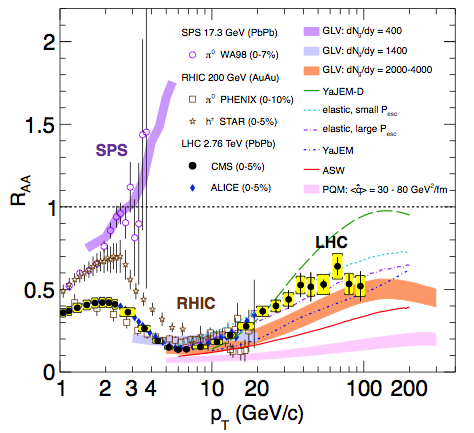
\includegraphics[width=0.65\textwidth]{pics/Raaplot}
        \caption[Measurements of the nuclear modification factor $R_{AA}$ in central heavy-ion collisions]{Measurements of the nuclear modification factor $R_{AA}$ in central heavy-ion collisions at three different center-of-mass energies, as a function of $\pt{}$, for neutral pions ($\pi^0$), charged hadrons ($h\pm$), and charged particles~\cite{Aamodt:2010jd, Aggarwal:2001gn, d'Enterria:2004ig, Adare:2008qa, Adams:2003kv}, compared to several theoretical predictions~\cite{Dainese:2004te, Vitev:2002pf, Vitev:2004bh, Salgado:2003gb, Armesto:2005iq, Renk:2011gj}. The error bars on the points are the statistical uncertainties, and the yellow boxes around the CMS points are the systematic uncertainties. The bands for some of the theoretical calculations represent their uncertainties~\cite{CMS:2012aa}.}
        \label{fig:Raa}
\end{figure}

If the medium has no effect on high $\pt{}$ particles the nuclear modification factor should be 1. As seen in Fig.~\ref{fig:Raa} $R_{AA}$ at RHIC and LHC has been observed to be as low as 0.2, which is a clear signal that jet quenching is happening. However, the physical interpretation is not that 80 \% of high momentum tracks disappear, rather they are shifted to smaller momenta. The relation between the shift in momentum and $R_{AA}$ depends on the steepness of the $\dd{N}/\dd{\pt{}}$ spectra. At LHC energies the spectrum is flatter and thus the same $R_{AA}$ value as in RHIC requires a larger momentum shift, which results from the larger temperature of the medium at LHC. 

The reaction plane dependence of inclusive particle $R_{AA}$ demonstrates that energy loss is path length dependent~\cite{Adler:2006bw}, as expected from models. The path length can be affected by collisions centrality and system size. However, the temperature and lifetime of the QGP also changes with changing centrality and system size. Thus to study different path lengths the angle relative to the reaction plane gives the cleanest signal, as the properties of medium remain the same. Additionally it was concluded that there is no suppression for path lengths below $\mathrm{L} = \unit[2]{fm}$. Similar indications about path length dependence are given by jet $v_2$ both at RHIC~\cite{Adare:2013wop} and at LHC~\cite{Abelev:2012di,Chatrchyan:2012xq}. 



 %Naturally jet quenching depends on the path lengths through the medium.

%\subsubsection*{Theory of jet quenching}


%After the hard partons are created they escape the medium before a thermal equilibrium is reached. Thus they are not part of the pressure-driven collective expansion. Instead high momentum yield is suppressed because of energy loss in the medium. When propagating through the medium these partons lose energy as they pass through the medium. This is referred to as jet quenching. Jet quenching depends on the path lengths through the medium. Thus anisotropy in this region is mainly dependent on the collision geometry and density of medium.


%The energy loss of partons in medium is mainly due to QCD bremsstrahlung and to elastic scatterings between the parton and the medium. 


\subsubsection*{QED Bremsstrahlung}

Many of the energy loss models exploit the analogy between the QCD interaction of parton propagating through the coloured medium and the QED energy loss of electron propagating through material. An electron propagating through matter loses its energy by photon Bremsstrahlung radiation. In the simplest case, each individual scattering center results in a single emission of a photon. This is known as the Bethe-Heitler regime~\cite{BetheHeitler}. The energy spectrum of radiated photons $\nicefrac{\dd N}{\dd E}$ is, in this case, proportional to $\nicefrac{1}{E}$. However, the Bremsstrahlung photon, can be radiated only when the distance between the scattering centers is larger than the formation length. In the limit, when the scattering centers are closer than the formation length, the Bremsstrahlung process is suppressed. This phenomenon is known as the Landau-Pomeranchuk-Migdal (LPM)~\cite{Landau:1953um,Migdal:1956tc} suppression. The radiated spectrum in this regime is proportional to $\nicefrac{1}{\sqrt{E}}$.

Lower energy photons are further suppressed by the destructive interference leading to the suppression of Bremsstrahlung photons of $E < \gamma \omega_p$, where $\omega_p$ is the plasma frequency of the radiator. This is knows as Dielectric suppression. The photon energy distribution in this regime is proportional to the energy of the photon. A schematic view of the effect of these three regimes is shown in Fig.~\ref{fig:bremsstrahlung}.

\begin{figure}[htb]
\centering
\includegraphics[height=2in]{pics/BremsstrahlungElectron}
\caption[Photon spectrum]{ The expected bremsstrahlung spectrum for a electron propagating through material.  ~\cite{Bosted1993QuantummechanicalSO}. }
\label{fig:bremsstrahlung}
\end{figure}

\subsubsection*{QCD}
In QCD the radiative energy loss mechanism is given in terms of the transport coefficient $\left<\hat q\right>$, which describes the average momentum transfer between the medium and parton~\cite{jetBroadeningPpb1}. The exact definition of this depends on the theoretical formalism used to describe the energy loss mechanism. 

The simplest energy loss process is elastic QCD scattering off the medium partons. In elastic scatterings the recoil energy of the scattered partons are absorbed by the thermal medium, which reduces the energy of the initial parton. The mean energy loss from elastic scatterings can be estimated by

\begin{equation}
\left<\Delta E\right>_{\mathrm{el}}=\sigma \rho L \left<E\right>_{\mathrm{1\,scatt}}\propto L,
\label{eq:elastic}
\end{equation}

\noindent where $\sigma$ is the interaction cross section and $\left<E\right>_{1 scatt}$ is the mean energy transfer of one individual scattering~\cite{Majumder:2010qh}. This assumption holds if the mean energy is independent of the total energy of the parton ($E$). The transport coefficient of elastic scattering, $\left< \hat q_\mathrm{el}\right> = \nicefrac{\left< \Delta E\right>}{L}$, is defined as the mean energy los per unit path length.

Another energy loss mechanism is medium-induced radiation. In QCD this radiation is mainly due to the elementary splitting processes, $q\rightarrow qg_r$ and $g\rightarrow gg_r$. Assuming that the parton is moving with the speed of light radiation energy loss can be estimated by

\begin{equation}
\left<\Delta E\right>_{rad}\propto T^3L^2,
\label{eq:radiative}
\end{equation}

\noindent where $L$ is the length of the medium and $T$ is its temperature~\cite{Dominguez:2008vd}. The different exponents of $L$ in equations \ref{eq:elastic} and \ref{eq:radiative} indicate that radiative energy loss is dominant over elastic energy loss.


There are several models that attempt to describe the nature of the energy loss mechanism. The most used models can be divided into four formalisms.
%
%\begin{itemize}
%\item Thermal effective theory formulation (AMY)~\cite{Arnold:2001ms, Arnold:2002ja}
%\item Opacity Expansion ((D)GLV/WHDG and ASW-SH)~\cite{Salgado:2003gb, Gyulassy:2000er, Gyulassy:1999zd, Wiedemann:2000za} 
%\item Higher Twist approach~\cite{Wang:2001ifa, Majumder:2009zu} 
%\item Multiple soft scattering approximation BDMPS-Z (ASW-MS)~\cite{Baier:1996kr, Zakharov:1996fv, Baier:1998kq, Salgado:2003gb}
%\end{itemize}

In the Gyulassy-Levai-Vitev (GLV)~\cite{Gyulassy:1999zd} opacity expansion model
 the radiative energy loss is consiered on a few scattering centers $N_{scatt}$. The radiated gluon is constructed by pQCD calculation as summing up the relevant scattering amplitudes in terms of the number of scatterings. Another approach into opacity expansion is the ASW model by Armesto, Salgado and Wiedermann~\cite{Wiedemann:2000za}.

Thermal effective theory formulation by Arnold, Moore and Yaffe (AMY)~\cite{Arnold:2001ms} uses dynamical scattering centers. It is based on leading order pQCD hard thermal loop effective field theory. This model assumes that because of the high temperature of the plasma the strong coupling constant can be treated as small. The parton propagating through the medium will lose energy from soft scatterings and hard scatterings.

The above models calculate the energy loss while the parton propagates through the medium, focusing on the pQCD part. The higher twist (HT) approach by Wang and Guo~\cite{Wang:2001ifa} implements the energy loss mechanism in the energy scale evolution of the fragmentation functions.

The last category is formed by the Monte Carlo methods. The PYTHIA event generator~\cite{pythia} is widely used in high-energy particle physics. Two Monte Carlo models based on PYTHIA describing the energy loss mechanism are PYQUEN~\cite{Lokhtin:2005px} and Q-Pythia~\cite{Armesto:2009zc}. Other Monte Carlo models include JEWEL~\cite{Zapp:2008gi} and YaJEM~\cite{Renk:2009nz}. 


%\subsubsection*{Discovery of jet quenching via leading hadron suppression}
%First evidence of jet quenching comes from observing high $\pt{}$ tracks, i.e. the leading hadrons.
%Jet quenching in heavy-ion collisions is usually quantified with the nuclear modification factor $R_{AA}$, which is  is defined as
%%the yield in heavy-ion collisions divided by the yield in proton-proton collisions and scaled by the The nuclear modification factor
%
%\begin{equation}
%R_{AA}\left(\pt{}\right) = \frac{(1/N_{AA}^{evt})\dd {N^{AA}}/\dd {\pt{}}}{\left< N_{coll}\right> (1/N_{pp}^{evt})\dd {N^{pp}}/\dd {\pt{}}}\label{eq:raa}
%\end{equation}
%\noindent where $\dd{N^{AA}}/\dd{\pt{}}$ and $\dd{N^{pp}}/\dd{\pt{}}$ are the yields in heavy-ion and proton-proton collisions, respectively and $\left< N_{coll}\right>$ is the average number of binary nucleon-nucleon collisions in one heavy-ion event. The number of binary collisions can be calculated from the Glauber model as shown in Sec.~\ref{sec:glauber}. From the point of view of direct production a heavy-ion collision can be estimated relatively well to be only a series of proton-proton collisions. 
%
%If the medium has no effect on high $\pt{}$ particles the nuclear modification factor should be 1. At RHIC and LHC this has been observed to be as low as 0.2 because of jet quenching. Measurements of $R_{AA}$ from different sources are shown in Fig.~\ref{fig:Raa}
%
%\begin{figure}[hbt]
%	\centering
%                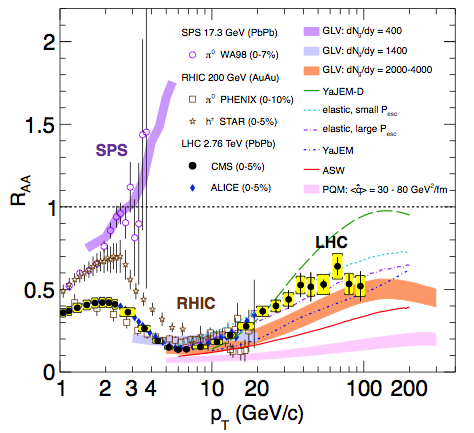
\includegraphics[width=0.65\textwidth]{pics/Raaplot}
%        \caption[Measurements of the nuclear modification factor $R_{AA}$ in central heavy-ion collisions]{Measurements of the nuclear modification factor $R_{AA}$ in central heavy-ion collisions at three different center-of-mass energies, as a function of $\pt{}$, for neutral pions ($\pi^0$), charged hadrons ($h\pm$), and charged particles~\cite{Aamodt:2010jd, Aggarwal:2001gn, d'Enterria:2004ig, Adare:2008qa, Adams:2003kv}, compared to several theoretical predictions~\cite{Dainese:2004te, Vitev:2002pf, Vitev:2004bh, Salgado:2003gb, Armesto:2005iq, Renk:2011gj}. The error bars on the points are the statistical uncertainties, and the yellow boxes around the CMS points are the systematic uncertainties. The bands for some of the theoretical calculations represent their uncertainties~\cite{CMS:2012aa}.}
%        \label{fig:Raa}
%\end{figure}
%
%
%The nuclear modification factor can also be used to quantify anisotropy. In the study of anisotropy $R_{AA}$ in-plane and out-of-plane can be compared, where plane refers to the plane defined by the impact parameter and the beam direction. The distance traveled through medium is largest out-of-plane which leads to stronger suppression in this direction. The nuclear modification factor as a function of $\Delta\phi=\phi-\psi_n$ is given by
%
%\begin{eqnarray}
%R_{AA}\left(\Delta\phi, \pt{}\right) &=& \frac{(1/N_{AA}^{evt})\dd {^2N}^{AA}/d\Delta\phi \dd {\pt{}}}{\left< N_{coll}\right> (1/N_{pp}^{evt})\dd {N^{pp}}/\dd {\pt{}}} \approx \frac{\dd {N^{AA}}/\dd {\pt{}}\left( 1+2\cdot v_2\cos{(2\Delta\phi)} \right)}{\left< N_{coll}\right> \dd {N^{pp}}/\dd {\pt{}}} \nonumber \\ &&\nonumber\\
%&=& R_{AA}^{incl}(\pt{}) \left( 1+2\cdot v_2\cos{(2\Delta\phi)} \right).
%\label{eq:raaandv2}
%\end{eqnarray}	
%
%The yield of proton-proton collisions is independent of the reaction plane and the yield in heavy-ion collisions is modulated by the second harmonics. In Eq. (\ref{eq:raaandv2}) $R_{AA}$ is approximated only up to the second harmonics.
%From \eq{eq:raaandv2} it follows that
%
%\begin{equation}
%\frac{R_{AA}\left(0, \pt{}\right)-R_{AA}\left(\pi/2, \pt{}\right)}{R_{AA}^{incl}(\pt{})} \approx \frac{R_{AA}^{incl}(\pt{}) \left(1+2 \cdot v_2-(1-2 \cdot v_2) \right)}{R_{AA}^{incl}(\pt{})} = 4 \cdot v_2
%\label{eq:raaandv2result}
%\end{equation} 
%%At high-$\pt{}$, the pQCD processes are dominant, hence the $v_n$ (or $R_{AA}(\Delta\phi, \pt{})$) characterize the path length-dependence of the energy loss process. 
%The observed $R_{AA}\left(\Delta\phi, \pt{}\right)$  from PHENIX measurements in Au-Au collisions at $\sqrt{s}=200\gev$~\cite{PhysRevC.80.054907} is compared to $R_{AA}$ using $v_2$  via \eq{eq:raaandv2} in Fig.~\ref{fig:RAAv2}. They agree very well within the statistical errors for all centrality and $\pt{}$ bins.
%\begin{figure}[htb]
%	\centering
%                \includegraphics[width=0.5\textwidth]{pics/RAAandv2Correlation}
%        \caption[A comparison between observed $R_{AA}\left(\Delta\phi, \pt{}\right) $ and $R_{AA}$ using $v_2$]{ A comparison between observed $R_{AA}\left(\Delta\phi, \pt{}\right) $ and $R_{AA}$ using $v_2$ from PHENIX measurements of Au-Au collisions at $\sqrt{s}=200\gev$. On the X-axis is the measured $R_{AA}\left(\Delta\phi,\pt{}\right)$. On the y-axis is the inclusive $R_{AA}$ multiplied by  $1+2v_2\cos\left(\Delta\phi\right)$~\cite{PhysRevC.80.054907}.}
%        \label{fig:RAAv2}
%\end{figure}
%
%At high-$\pt{}$, the pQCD processes are dominant, hence the $v_n$ (or $R_{AA}(\Delta\phi, \pt{})$) characterize the pathlength-dependence of the energy loss process. ~\ref{fig:highpt}
%
%Jet quenching is not the only high $\pt{}$ phenomenon studied in heavy-ion collisions. Another property is jet fragmentation. The high momentum parton created in the initial collision fragments into a number of partons with smaller $\pt{}$. Jet fragmentation occurs also in proton-proton collisions in the vacuum, but it can be modified due to the presence of the medium. In order to study the jet fragmentation function ($D(z)$, where $z= \pt{}^h/\pt{}^{part}$) modification due the medium, we use the two-particle correlations. The particle yield can be extracted from the correlation function. The background from the flow processes is correlated and needs to be subtracted to get the particle yield associated only with the jet. The ratio of the jet yields in Au-Au and p-p collision $I_{AA} = {Y^{Au+Au}}/{Y^{p+p}}$ characterizes the jet fragmentation modification \cite{Aamodt:2011vg}. $I_{AA}$ probes the interplay between the parton production spectrum, the relative importance of quark-quark, gluon-gluon and quark-gluon final states, and energy loss in the medium~\cite{missing}.
%
%
%\begin{figure}[ht]
%\centering
%\includegraphics[width=0.9\textwidth]{pics/fig2_vn_exp-11543.pdf}
%\caption[Elliptic flow, $v_2$ from $\pt{}=1$ to $60\gevc$]{} %Elliptic flow, $v_2$, as a function of the charged particle transverse momentum from $1$ to $60\gevc$ with $\left|\eta\right|<1$ for six centrality ranges in Pb-Pb collisions at $\snn=2.76\tev$, measured by the CMS experiment.~\cite{Chatrchyan:2012xq}. }
%\label{fig:highpt}
%\end{figure}



\subsubsection{New paradigm of jet Quenching}
%As described in the previous section there have been many experimental evidences of jet energy loss, such as the suppression of inclusive hadron spectra at high transverse momentum~\cite{Adcox:2001jp,Adams:2003im,Arsene:2003yk,Khachatryan:2016odn,Acharya:2018qsh}, the modification of back-to-back hadron-hadron~\cite{Adare:2007vu,Aamodt:2011vg} and direct photon-jet correlations~\cite{Adare:2012qi}, and the modification of reconstructed jet spectra~\cite{Adam:2015ewa} and jet substructure~\cite{Sirunyan:2018qec,Chatrchyan:2014ava,Acharya:2018uvf}, as compared to the expectations from elementary proton-proton collisions.


As described in the previous sections the first indications of jet quenching, such as $R_{\mathrm{AA}}$, looked essentially at the leading hadrons of jets, the hard part, ignoring the soft scale part of jet phenomena. However, experimental methods have since improved; jet reconstruction algorithms have become reliable in the LHC era. Instead of the leading hadron we can study the entire jet shower and its structure. In jet observables one must consider what happens to the lost energy. Radiated gluons may end up being clustered with the jet, depending on the radiation angle, the parameters of jet reconstruction and whether the gluon reaches equilibrium with the medium or not. Thus the suppression on the jet level is expected to be smaller. Figure~\ref{fig:jetraa} shows jet $R_{AA}$ in central \PbPb collisions measured by ALICE,ATLAS and CMS and indeed jet $R_{AA}$ is about 0.5 instead of 0.2. %This raises the conceptual question, what counts as being part of the jet.  If a gluon radiated from the jet thermalises with the medium, is it a part of the jet or the medium?


%The first evidence of jet quenching in reconstructed jets at the LHC was observed by measuring the dijet asymmetry, $A_j$ ~\cite{Connors:2017ptx}.  


\begin{figure}
\centering
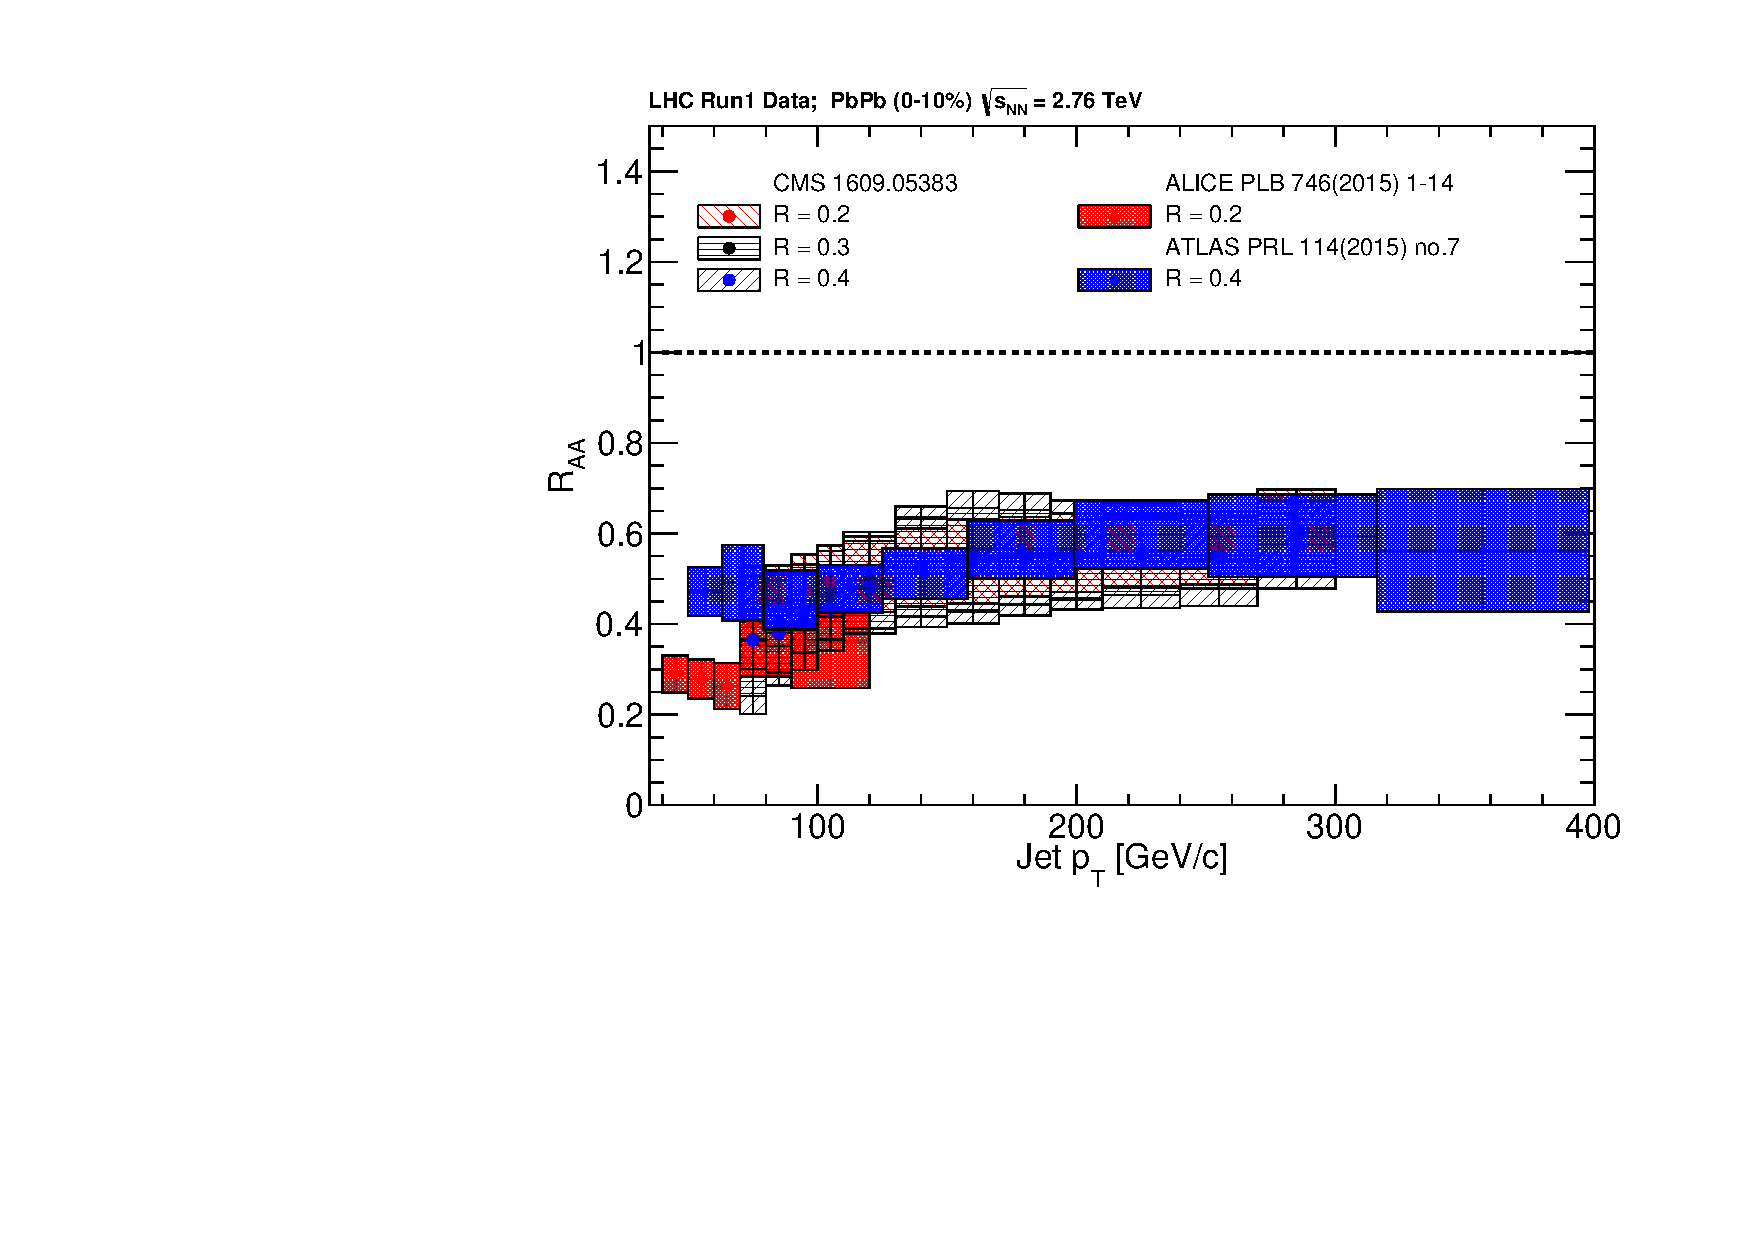
\includegraphics[height=2.4in]{figures/LHC_Run1_RAA_comparison_cent010.pdf}
\caption{Reconstructed anti-$\kt{}$ jet $R_{AA}$ from ALICE~\cite{Adam:2015ewa} with $R = 0.2$ for $\left| \eta \right| < 0.5$, ATLAS~\cite{Aad:2014bxa} with $R = 0.4$ for $\left| \eta \right| < 2.1$, and CMS~\cite{Khachatryan:2016jfl} with R = 0.2, 0.3 and 0.4 for $ \left| \eta \right| < 2.0$. The ALICE and CMS data are consistent within uncertainties while the ATLAS data are higher. The experiments use slightly different methods in selecting jets and subtracting the underlying event contribution. Compared to ALICE and CMS the ATLAS technique could impose a survivor bias and lead to a higher jet RAA at low momenta. Figure from~\cite{Connors:2017ptx}}
\label{fig:jetraa}
\end{figure}

Thus, on the level of the reconstructed jet, energy loss manifests itself as broadening and softening of the jet. This is seen for example in jet-hadron correlations. Figure~\ref{fig:jethadron} shows $\Delta \eta$ correlations with the leading jet. $\Delta \phi$ correlations have similar trends. Jets in \PbPb are observed to be broader, with the greatest increase in the width for low momentum associated particles. This is consistent with expectations from partonic energy loss. These studies found that the subleading jet was broadened even more than the leading jet, indicating a bias towards selecting less modified jets as the leading jet.
Jet hadron correlations have also been studied at RHIC with similar conclusion~\cite{Adamczyk:2013jei}.


\begin{figure}
\centering
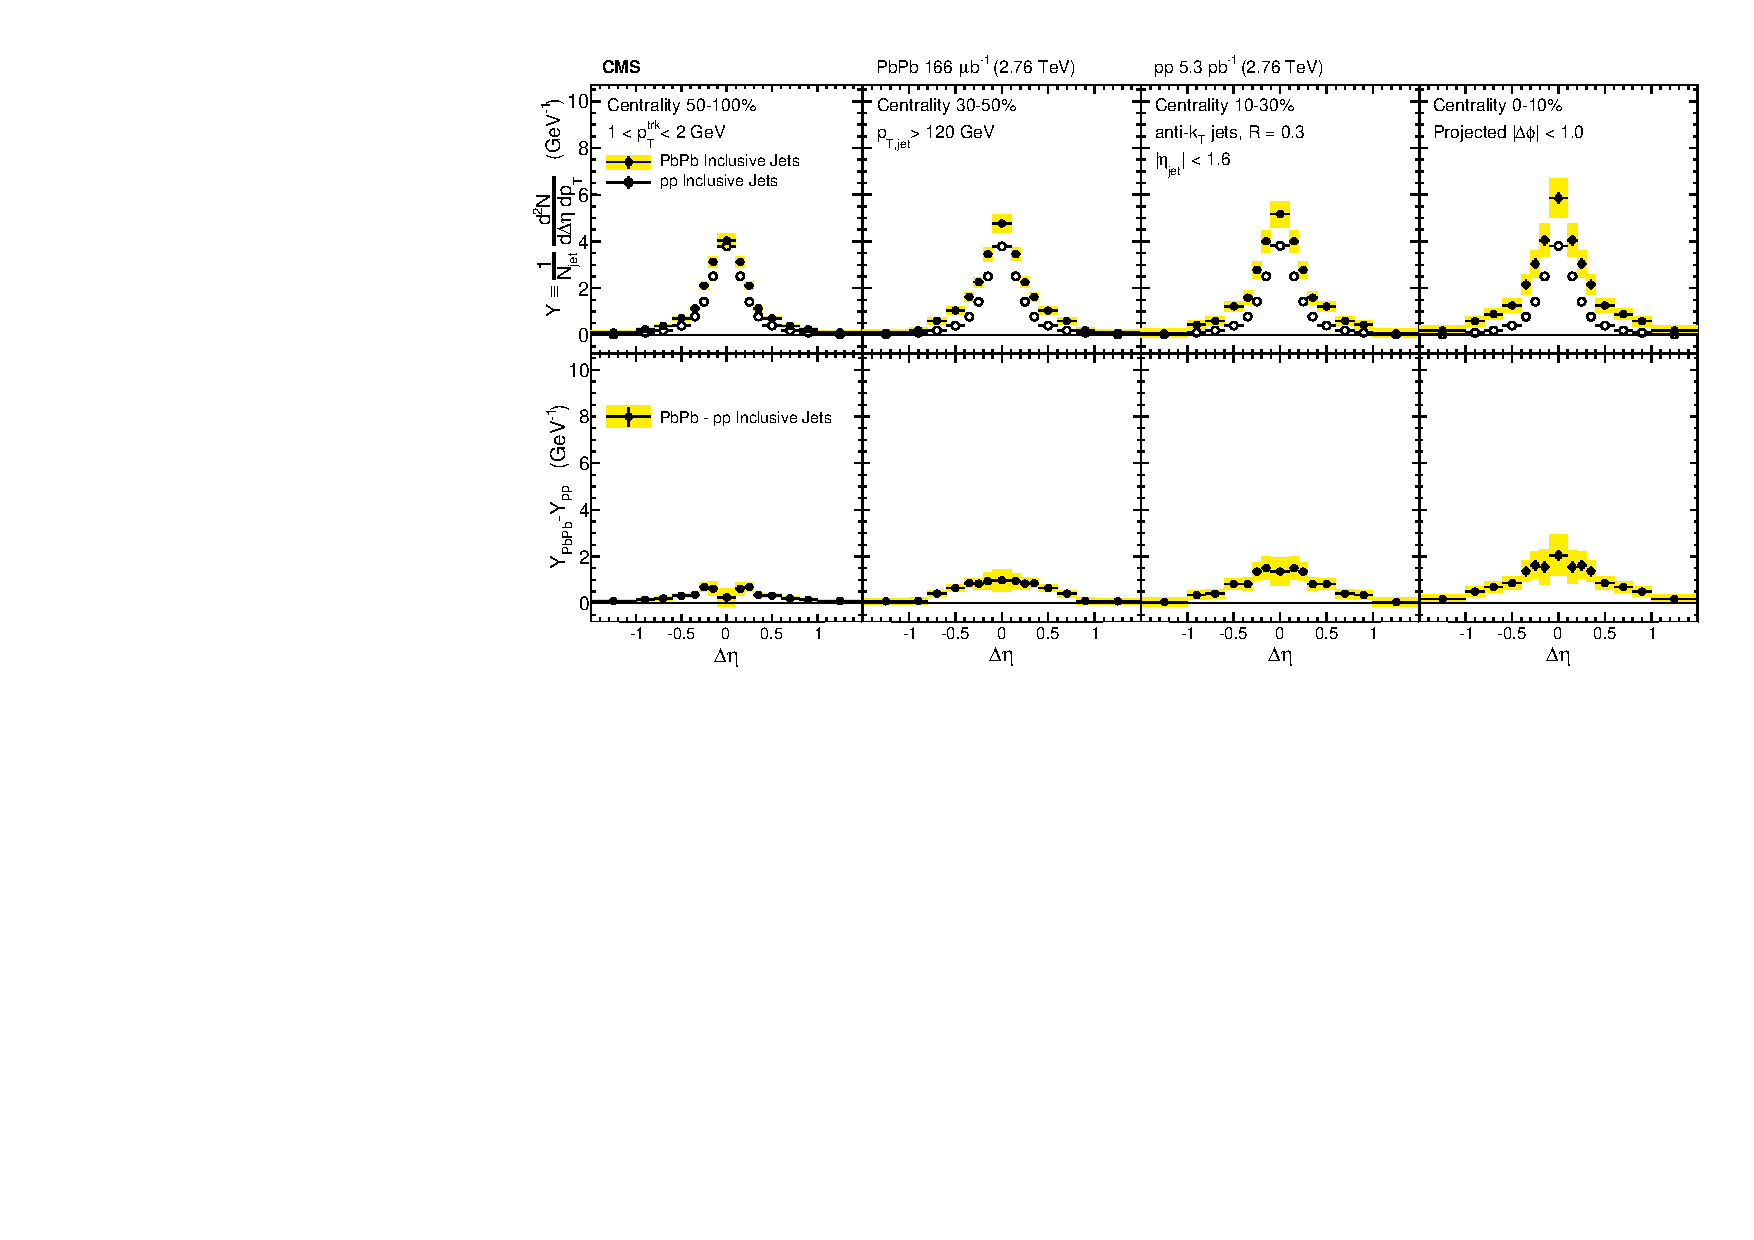
\includegraphics[height=2.4in]{figures/TrackJetCMS-HIN-14-016_Figure_003.pdf}
\caption{Measurement by CMS~\cite{Khachatryan:2016erx}. Symmetrized $\Delta \eta$ distributions correlated with \PbPb and \pp inclusive jets with $\pt{}>\unit[120]{\gev}$ are shown in the top panels for tracks with $1 < \pt{} < \unit[2]{\gev}$. The difference between per-jet yields in \PbPb and \pp collisions is shown in the bottom panels. These measurements indicate that the jet is broadened and softened, as expected. The effect is stronger in more central collisions.  $\Delta \phi$ correlations have similar trends.}
\label{fig:jetraa}
\end{figure}




\subsubsection*{Phase-space view of the medium modified parton cascade}
The new paradigm in jet quenching in heavy-ion collisions involves multi-scale problems~\cite{Kurkela:2014tla,Tachibana:2018yae}. The elementary scattering and the subsequent branching process down to non-perturbative scales are dominated by hard scales in the vacuum as well as in the medium. Soft scales, of the order of the temperature of the medium, characterise the interactions of soft partons produced in the shower with the QGP. Soft scales also rule hadronisation, which is expected to take place in vacuum for sufficiently energetic probes, even though some modifications can persist from modifications of colour flow~\cite{Aurenche:2011rd,Beraudo:2011bh,Beraudo:2012bq}. Understanding the contributions from the different processes to the jet shower evolution in medium and their scale dependence is crucial to to constrain the dynamics of jet energy loss in the expending medium, the role of colour coherence~\cite{CasalderreySolana:2012ef}, and fundamental medium properties like temperature dependent transport coefficient~\cite{DEramo:2012uzl,Ayala:2016pvm}.

\begin{figure}[tbp]
\centering
\begin{subfigure}{0.45\textwidth}
\includegraphics[width=0.99\textwidth]{figures/regions4.eps}
%\caption[]{Illustration of how a medium-modified parton cascade fills the phase space. Early stage vacuum radiation dominates phase space in the DGLAP region. Late stage, after exiting the medium, radiation dominates the Late DGLAP regions.  }
%Parametrically accurate picture of how a medium-modified parton cascade fills the phase space. At time $t$, quanta can be formed up to momentum scale $k_{\rm form}$ and they are formed with $O(1)$ probability per $\log p$ at lower scale $k_{\rm split}$. Quanta below $k_{\rm split}$ split further and their energy cascades to the thermal scale $T$ in less than an epoch $t$. Transverse Brownian motion moves quanta up to the angle $\theta_{\rm BR}(p)$ denoted by the thick purple line.  The Moli\`ere region at larger $\theta$ is dominated by rare large angle scattering. At even larger angle, there are $O(\alpha_s)$ quanta per double logarithmic phase space  from DGLAP 'vacuum' radiation, and for momenta below $k_{\rm split}$ these cascade within time $t$ to $T$. After the jet escapes the medium, the jet and the emitted fragments will undergo vacuum radiation. This late time vacuum radiation emitted by the original parton dominates at sufficiently small $\log \theta$  (regions marked ``late DGLAP'' and bounded by $\theta_{\rm vac}$ and $\theta_\alpha$),  whereas the late time radiation of the fragments dominates in the region  denoted by ``Vacuum cascade of the medium induced quanta''. }
%\label{fig:cascades}
\end{subfigure}
\begin{subfigure}{0.45\textwidth}
\includegraphics[width=0.99\textwidth]{figures/e-vs-th3.eps}
%\caption[]{The distribution of energy as a function of angle for a fixed $p > k_\mathrm{split}$. The  Medium induced radiation dominates around the angular scale $\theta_\mathrm{BR}$. The medium induced contributions (dashed lines) grow as a function of evolution time with respect to the vacuum one (dotted line). ~\cite{Kurkela:2014tla}.}
%\label{fig:edistribution}
\end{subfigure}
\caption{{\it Left}: Phase space view of dominant contributions in a medium-modified parton cascade. {\it Right} The distribution of energy as a function of angle for a fixed momentum with $p > k_\mathrm{split}$. Large angular scales $\theta > \theta_\mathrm{Mol}$ are dominated by DGLAP vacuum radiation from the leading parton at the scale $Q$. At $\theta < \theta_\alpha$ the energy density is dominated by vacuum radiation of the leading parton after it has degraded its energy propagating through the medium. Areas $\theta_\alpha < \theta < \theta_\mathrm{BR}$ and $\theta_\mathrm{BR} < \theta < \theta_\mathrm{Mol}$ are dominated by Brownian motion and rare large angle (Moli\`ere) scatterings with medium partons ~\cite{Kurkela:2014tla}.}
\label{fig:cascades}
\end{figure}

Let us now look at medium modification of jets in a $\log\left(p\right)-\log\left(\theta\right)$ plane as shown in ~\cite{Kurkela:2014tla}. The different momentum and angular scales are subject to different physical phenomena. Figure~\ref{fig:cascades} shows the relevant medium modification phenomena for different regions of the phase space at time $t$, when a jet propagates through a thermal cloud of temperature $T$. As in a practice jets propagate over a finite path-length $L$ in QCD matter, Fig.~\ref{fig:cascades} can be taken as a representation of the distribution of partonic jet fragments at moment $t \approx L$, when the jet escapes the medium.~\cite{Kurkela:2014tla}

The region marked as DGLAP is dominated by the primary vacuum splittings explained in section~\ref{sec:shower}. This region is determined by $\theta > \theta_\mathrm{vac}$ with

\begin{equation}
\theta_\mathrm{vac} \propto \nicefrac{1}{\sqrt{\pt{}}}.
\end{equation}


\noindent Medium-induced parton branching fills the $\log p$-$\log \theta$-plane from the bottom up (in $p$) and from the inside out (in $\theta$). This is because transverse momentum is acquired by Brownian motion in the medium, $k_\perp^2 \propto \hat q t$. The formation time constraint $t \geq \nicefrac{p}{k_\perp^2} \approx \nicefrac{p}{\hat q t}$ implies that medium-induced quanta can be formed in the region $p \leq k_\mathrm{form}$ where

\begin{equation}
k_\mathrm{form}\left(t\right) = \hat q t^2.
\end{equation}

\noindent For these splittees to survive without further splittings they must have 
\begin{equation}
p \geq k_\mathrm{split} \approx \alpha_s^2 k_\mathrm{form}\left(t\right) \approx \alpha_s^2\hat q t^2.
\end{equation} 

\noindent Thus the region marked as LPM in Fig.~\ref{fig:cascades} is filled by the primary medium-induced branchings. Fragments with $p \leq k_\mathrm{split}$ will have time to split further. An approximately equal splitting where both splittees get momentum $~\nicefrac{p}{2}$ from the parent will degrade energy the most. These splittees will undergo the next splitting in an even shorter time scale producing even softer fragments. Momenta can continue cascading all the way to the thermal scale $T$ of the medium within the same time scale within which the first splitting occurred. Thus filling the region marked as Medium cascade in Fig.~\ref{fig:cascade}. Similarly splittees from vacuum radiation can cascade inside the medium when they have $p \leq k_\mathrm{split}$, filling the bottom right corner of the $\log p$-$\log \theta$-plane.

%
%%\begin{equation}
%%\frac{\mathrm d P_\mathrm{find}\left(t\right)}{\mathrm d \log p} \propto \alpha_s \nicefrac{t}{t_\mathrm{form}}\left(p\right) \propto \alpha_s \hat q ^{\nicefrac{1}{2}} p^{-\nicefrac{1}{2}} t
%%\end{equation} 
%
%\noindent Not all quanta will stay where they were created. Those modes that have time to lose a significant fraction of their energy will cascade to a significantly lower scale $p$. For LPM-type radiation, the splitting that degrades energy the most is the hardest splitting. 
%
%The $\log p $ distribution has the same $\frac{1}{\sqrt{p}}$ dependence as in the LPM region
%
%\begin{equation}
%\frac{\mathrm{d}n}{\mathrm{d}\log p} = \frac{1}{p}\frac{\mathrm{d}\epsilon}{\mathrm{d}\log p} \approx \alpha_s \frac{\sqrt{\hat q t}}{\sqrt{p}}
%\end{equation}
%
%\noindent Also the quanta originating from the DGLAP region will undergo medium interactions that will make the quanta radiate and split. The distribution of radiation is the same as from any other mode. Above a certain momentum scale $k_\mathrm{split}$ the distribution of originating daughters is 
%
%
%\begin{equation}
%\frac{\mathrm d P_\mathrm{find}}{\mathrm d \log p \mathrm{d} \log \theta} \approx \alpha_s \frac{t}{t_\mathrm{split}\left(p\right)},
%\end{equation} 
%
%%\noindent Note that the ratio $\nicefrac{t}{t_\mathrm{split}}$ is smaller than 1 for nodes above $k_\mathrm{split}$ and therefore the number of daughters is smaller than the number of vacuum splitted quanta. Below $k_\mathrm{split}$ the cascade is similar to the medium cascade and the number of quanta become
%%
%%\begin{equation}
%%\frac{\mathrm{d}n}{\mathrm{d}\log p \mathrm{d} \log \theta} \approx \alpha_s \frac{t}{t_\mathrm{split}\left(p\right)}, \text{ for } p < k_\mathrm{split}\left(p\right)
%%\end{equation}


The angular distribution of the medium-induced radiation is driven by two mechanisms; Multiple soft scatterings give rise to transverse Brownian motion, which determines the distribution at small angles. The typical angle reached in the LPM region is 

\begin{equation}
\theta_\mathrm{BR}\left(p\right) \approx \frac{\sqrt{\hat q t}}{p}, \text{ for } k_\mathrm{form} > p > k_\mathrm{split},
\end{equation}

\noindent while in the medium cascade region of the phase space this becomes

\begin{equation}
\theta_\mathrm{BR}\left(p\right) \approx \left(\frac{T}{p}\right)^{\frac{3}{4}}
\end{equation}

\noindent Large angular scales cannot be reached by Brownian motion, but can arise from rare large angle scatterings with partons in the medium, described first by Molière~\cite{missing}. The result is that medium-induced radiation is predominantly located in the bands marked as Brownian motion, where $\theta_\alpha < \theta < \theta_\mathrm{BR}$, and Moli\`ere, where $\theta_\mathrm{BR} < \theta < \theta_\mathrm{Mol}$ in Fig.~\ref{fig:cascade}. 

The hard parton will naturally continue radiating after it leaves the medium. As there is no longer kinematic limits set by the time scale, the vacuum radiation can extend to smaller angular scales in the phase space. The results is that the regions, where $\theta<\theta_\alpha$, marked as Late DGLAP in Fig.~\ref{fig:cascade} will be dominated by the late time vacuum radiation. Naturally also the splittees from medium-induced radiation will undergo the late stage vacuum radiation phase, filling the triangular region with small $p$ and $\theta < \theta_\mathrm{\alpha}$.



\subsubsection*{Influence of jet on medium}
Energy loss of hard partons is well established by experimental observations. Naturally energy can't just disappear, but is transferred to daughter partons or the medium. For radiation that stays inside the jet cone energy loss manifests itself as softening and broadening. If a daughter parton loses energy and becomes equilibrated with the medium it may no longer be correlated with the parent parton. This energy would then be distributed at distances far from the jet cone. There is some evidence for out-of-cone radiation by CMS~\cite{Chatrchyan:2011sx}, but the interpretation is not clear. Other possible phenomena include the mach cone and Moliére scattering, but there is no experimental evidence for these. Evidence for all of these effects is difficult to find as the underlying event gives already a large and fluctuating background. Additionally its unclear how this energy would be different from the underlying event~\cite{Connors:2017ptx}.
